\documentclass{article}
\usepackage[margin=3.15cm]{geometry}
\usepackage{natbib}
\usepackage{amsmath}
\usepackage{amssymb}
\usepackage{amsthm}
\usepackage{hyperref}
\usepackage{xcolor}
\usepackage{lipsum}
\usepackage{graphicx}
\usepackage{bm}
\usepackage{booktabs}
\usepackage{soul}
\usepackage{algorithm2e}
% \usepackage{setspace}
% \doublespacing

\title{Multivariate Extreme Value Theory and Applications to Anomaly Detection}
\author{Peter Trubey}
\date{}

\newcommand{\bruno}[1]{\textcolor{blue}{#1}} % Bruno Sanso edits- blue
\newcommand{\findcite}{{\color{red} [Find Citation]}}
\newcommand{\needcite}{\findcite}
\newcommand{\makenote}[1]{{\color{red} #1}}
\newcommand{\Chi}{\mbox{\Large$\chi$}}
\newcommand{\norm}[1]{\left\lVert #1 \right\rVert}
\newcommand{\inorm}[1]{\norm{#1}_{\infty}}
\newcommand{\pnorm}[2]{\norm{#1}_{#2}}

\newtheorem{prop}{Proposition}

\DeclareMathOperator{\tr}{Tr}
\DeclareMathOperator*{\argmin}{arg\,min}
\DeclareMathOperator*{\argmax}{arg\,max}

\begin{document}

\maketitle
\thispagestyle{empty}
\begin{abstract}
  
In recent years much work has been done in exploring the definition and properties of an appropriate
  generalization of the univaraite generalized Pareto distribution for threshold exceedences to a
  multivariate setting.  This paper builds on the constructive definition of the multivariate Pareto
  presented in \cite{ferreira2014} that decomposes the vector of interest into independent radial and
  angular components; the latter supported on a particular manifold and containing only information
  relevant to the dependence structure of the distribution.  We motivate our analysis with a discussion
  of extreme analysis applications in atmospheric sciences, in particular using the integrated vapor
  transport (IVT) data for assessing atmospheric rivers.

In this paper, we propose a novel approach to parameterize this dependence structure and conduct
  inference upon it.  We then explore some opportunities afforded to us by a parametrically modelled
  dependence structure in classical multivariate extreme analysis.  Finally, we explore the efficacy
  of some anomaly detection methods made possible by the existence of such a distribution, adapted
  to the support of the angular component.

\makenote{Extend the abstract.  Highlight the importance of EVT as a tool to predict behavior of
    tails of a distribution.  Also talk about applications considered, and computational challenges.}
% EOF

\end{abstract}

\newpage

\tableofcontents
\thispagestyle{empty}

\newpage

\clearpage
\pagenumbering{arabic}


\section{Introduction}
In recent years much work has been done in the exploration of the definition and properties of an
  appropriate generalization of the \emph{univariate} generalized Pareto distribution for exceedences
  over a threshold, to a \emph{multivariate} setting.  For a short accounting of the topic, the work of
  \cite{rootzen2006} defines the generalized Pareto distribution, with further analysis on these classes
  of distributions presented in \cite{falk2008} and \cite{michel2008}.  A recent review of the state
  of the art in multivariate peaks over threshold modelling using generalized Pareto is provided in
  \cite{rootzen2018}.  \cite{ferreira2014} presents a constructive definition of the multivariate Pareto
  that decomposes the random vector into independent radial and angular components; the latter
  containing all and only information pertaining to the dependence structure of the random vector.
  Based on this definition, we present a novel approach for modelling that angular component, and thus
  the modelling the dependence structure of the random vector.

To motivate the topic and our proposed solution, we acknowledge the relevance of extreme analysis to
  climatological events.  Outcomes such as heat waves, extreme precipitation, storm surges, and
  such present a similar challenge to investigators, in that the events of interest can be very destructive,
  and occur in probability at the tail end of \emph{normal} behavior.  In this fashion, a model built
  to capture \emph{normal} behavior may struggle to adequately represent extreme behavior.  More
  specialized tools become necessary; especially so in a time of intensifying extreme weather
  events~\citep{jentsch2007,vousdoukas2018,li2019}.  To this end, we use the integrated water vapor
  transport (\emph{IVT}) data for observing atmospheric rivers as an example application for our proposed method.

The first topic of the dissertation will concern the development of a model for multivariate extreme analysis,
  choosing to represent the dependence structure of multivariate Pareto using the projection of independent
  Gamma random variables onto the support of the angular component.  Analysis of this distribution follows.
  The second topic provides a review of the field of anomaly detection, and concerns contributions
  to the intersection of anomaly detection and extreme analysis that can be made using our model.
  The final topic discusses computational developments, and the application of extreme
  analysis--particularly our model--at scale.

The organization of the advancement document proceeds as follows:
  Section~\ref{sec:background} explains relevant background information; beginning with an overview of
  IVT, as well as a brief summary of field of extreme value theory.  Here we explain the specific space
  that the angular component of the multivariate Pareto is supported on. In Section~\ref{sec:methodology},
  we explore the difficulties in establishing a distribution on that support.  We introduce a family of
  manifolds that converge to our target space, and introduce a family of distributions supported on those
  manifolds.  In Section~\ref{sec:evaluation} we discuss what criteria are available to evaluate model
  fidelity, for the models we propose.  The nature of the space on which we build our model renders Euclidean
  distance inappropriate for model evaluation, so we discuss by what method we establish its replacement.
  Section~\ref{sec:results} presents metrics of model fidelity on simulated data for the proposed models,
  along with such metrics as evaluated on the IVT data.  In Section~\ref{ref:applications}, we discuss
  some of the possibilities afforded to us by such a parametric representation, and produce examples
  based on the IVT data, including pairwise extremal dependence coefficients, along with conditional
  survival curves using the posterior predictive distribution generated from our best model.
  Section~\ref{sec:anomaly} introduces the topic of anomaly detection, and provides a brief background
  of the field.  We also offer some methods of anomaly detection suited to multivariate EVT, and
  particularly suited to the statistical model we proposed. A preliminary analysis of our anomaly
  detection methods versus selected canonical methods is completed on simulated data, which shows
  our methods to be competitive.  In Section~\ref{sec:scale}, we discuss by what means we can scale
  this model to a large number of dimensions, along with a large number of observations.  Finally, we
  conclude, and present a timeline for the remaining work for the dissertation.

  % EOF


\section{Background}
\label{sec:background}

\subsection{Atmospheric Rivers}
\label{subsec:ar}
Atmospheric rivers are temporary events, where large elongated regions of high concentrations of
  water vapor are developed in the atmosphere and carry huge amounts of water potentially thousands
  of miles.  The amount of water in transit during these events dwarfs that of terrestrial rivers.
  For the targeted region, the atmospheric river can represent a significant portion of the
  precipitation the region will experience.  Such events are thus of great interest to meteorologists,
  as well as farmers, \makenote{expand and cite}.

One metric by which we might identify and declare atmospheric rivers is the integrated water vapor
  transport, or \emph{IVT}.  This value represents the total amount of water
  vapor being transported in an atmospheric column--that is, a column of the troposphere of particular
  size. These values can be measured by dropsondes, but the values we are using are estimated as part
  of a data product\makenote{needs citation}.  An observation from these data
  \makenote{IVT is a product, it is not observed.  Fix!} includes a reading (estimated
  or measured) at grid cell at a period in time; where a grid cell specifies the surface of the
  earth under the atmospheric column.  Our specific data comes from the coast of California,
  with daily readings of IVT covering 30 years, omitting leap days.  \makenote{Give more info, look into other paper}.
  We have two such datasets, in
  differing spatial resolutions.  The lower resolution splits the coast of california into 8 grid
  cells, while the higher resolution does so into 46 grid cells.

As IVT tracks water vapor in the atmosphere, extreme values in IVT can lead to
  extreme precipitation events.  Atmospheric rivers are necessary events, in that they carry the
  bulk of precipitation that California recieves, but extreme precipitation events can be extremely
  destructive as well.  Thus, we are interested in the distribution of extreme precipitation events,
  including their depenedence structure.  This tells us about the probability of jointly extreme
  events--where IVT is extreme in two or more grid cells, as well as identifying particular
  configurations of IVT that may be anomalous.  In California, groundwater is a managed resource.
  Extreme precipitation events significantly affect groundwater, so anomalous precipitation events
  can produce anomalous configurations of groundwater, leading to destructive flooding.

We are specifically interested in extremal dependence--the relationship between the upper tails of
  dimensions of the distribution.  In this case, that means the relationship between extreme values
  in different grid cells.  We are going to be looking at point-in-time behavior rather than
  considering the time series nature of the data--that relationship may come later.

As we are interested in the extremal dependence, it makes sense that we would choose to represent
  this data using tools from extreme value theory.  Extreme value theory, or \emph{EVT}, seeks to
  model and assess probability of observing extreme events.  Such a topic is applicable generally,
  but it finds particularly strong use among such fields as finance \citep{allen2013},
  climatology \citep{trepanier2018}, and insurance \citep{beirlant1994}.  In these fields, extreme
  events may represent significant loss to the body commissioning the study.  For instance, an
  insurance company might commission a study on extreme weather events, as an extreme weather event
  localized to a particular region could cause a spike in claims from that region.  Extreme value
  theory offers us a tool set for making inference about the tails of a distribution, without having
  observed said tails.  For
  instance, with an extreme weather event like flooding, we can make predictions about return
  levels--the average time until an observation of a particular magnitude occurs--without having seen
  an observation of that magnitude, or having observed that long.  In the context of our motivating
  example, extreme values in the IVT may represent the formation of an atmospheric river, which has
  dramatic effects on precipitation and ground water.  The formation of an IVT may lead to flooding
  and other negative effects, but is also contributes necessary water for irrigation and agriculture.
  Development of statistical tools regarding these extreme events becomes necessary for making informed
  decisions.

\subsection{Univariate EVT - Maxima}
\label{subsec:unietvmax}
Regarding the asymptotic behavior of extreme events, there are a couple major strategies for conducting
  inference--developing probabilistic estimates of extreme behavior.  First developed is the theory
  of a limiting distribution on maxima--the largest observation from a sample.  For a sample $\bm{x}$
  where $\bm{x} = (x_1,\ldots,x_n)$ represents a sequence of $n$ independent random variables from a
  distribution function $F$, the distribution of the maximum $M_n$ of this sequence can be derived
  as:
  \begin{equation*}
    \begin{aligned}
      \text{Pr}\left[M_n\leq z\right] &= \text{Pr}\left[X_1 \leq z, \ldots, X_n \leq z\right]\\
        &= \text{Pr}\left[X_1\leq z\right]\times\ldots\times\text{Pr}\left[X_n\leq z\right]\\
        &= F(z)^n.
    \end{aligned}
  \end{equation*}
  In situations where $F$ is unknown, we can seek to approximate the behavior of $F^n$ as
  $n\rightarrow\infty$.  To ensure this does not degenerate to a point mass, we need to consider a
  standardized sequence of maxima. If this sequence stabilizes as $n$ increases, the a limiting
  distribution exists.  More specifically, if there exists some sequence of constants $a_n > 0$, $b_n$
  such that:
  \begin{equation*}
    \text{Pr}\left[\frac{M_n - b_n}{a_n} \leq z\right] \stackrel{d}{\rightarrow} G(z)
  \end{equation*}
  as $n\rightarrow\infty$, then $G$ is a max-stable distribution, and $F$ is in the domain of
  attraction of that max stable distribution.  Maurice Fr{\'e}chet \citep{frechet1927} originates the
  field, identifying two limiting forms of max-stable distributions, which would become known as the
  Fr{\'e}chet and Weibull distributions. \cite{weibull1951} expands the analysis of the Weibull
  distribution.  \cite{fisher1928}, in what is now called the \emph{Fisher-Tippett Theorem}, identifies
  the Fr{\'e}chet and Weibull distributions, along with an as then unnamed third form, as the three
  limiting forms of the distribution of the maxima of a sample.  \cite{gumbel1935,gumbel1942} offers
   an analysis of that third form, now known as the Gumbel distribution.  Later works, including
   \cite{jenkinson1955} reparameterize all three forms as special cases of a single unifying form,
   the generalized extreme value distribution, \emph{GEV}:
  \begin{equation*}
    \label{eqn:gev}
    F(m \mid \mu, \sigma, \xi) = \exp\left\lbrace-\left[1 + \xi\left(\frac{x - \mu}{\sigma}\right)\right]_{}^{-1/{\xi}}\right\rbrace.
  \end{equation*}
  Thus distributions in the domain of attraction of an EVD (Gumbel, Fr{\'e}chet, or Weibull) will be
  in the domain of attraction of the GEV.

As this distribution specifies asymptotic behavior for the maximum of a set of observations,
  inference assuming this distribution requires we that specify some block of data, and for the block
  report only the maximum.  A series of these blocks yielding a series of maxima allows us to conduct
  inference about the parameters of the distribution.  Taking only the
  maximum in a block of observations necessarily leads to the reduction of our sample size by a factor
  of $1/\text{block size}$. In problems where the data occur in natural blocks, such as an hourly time
  series where a natural block might be a day, this might be appropriate.  There is an implicit
  violation of the assumption of independence within a block, in most cases, but that violation is
  generally ignored. In data without a natural block, it may be difficult to justify an induced
  artitifial block. Moreover, by reducing available information, retaining only one datum for each
  block increases the variability of the parameter estimates.

\subsection{Univariate EVT - Peak Over Threshold}
\label{subsec:univevtpot}
The \emph{Pickands-Balkema-de Haan Theorem}~\citep{balkema1974,pickands1975} offers us another means
  of conducting inference that will be less wasteful of data.  If the original distribution $F$ is
  in the domain of attraction of the GEV, then excesses over a high threshold $u$ can be well modelled
  using the Generalized Pareto distribution.  Again, let $X$ follow some distribution function $F$.
  It follows that:
  \begin{equation*}
    \text{Pr}\left[X > u + y\mid X > u\right] = \frac{1 - F(u + y)}{1 - F(u)}
  \end{equation*}
  for $y > 0$.  If $F$ is in the domain of attraction of an EVD, then
  \begin{equation*}
    \lim\limits_{u\to u^{\prime}}\text{Pr}\left[X > u + y\mid X > u\right] = H(y)
  \end{equation*}
  where $u^{\prime}$ represents some upper boundary of $X$ has a functional form--the survival
  function of a Pareto distribution. We approximate this asymptotic relationship by setting some
  large threshold $u$, and then threshold exceedences $Y = X - u$ are modelled under the distrribution
  function
  \begin{equation*}
    \label{eqn:gp}
    H(y) = 1 - \left(1 + \xi\frac{y}{\sigma}\right)^{-\frac{1}{\xi}}.
  \end{equation*}
  This defines the generalized Pareto family of distributions.  Thus, if block maxima have a
  limiting distribution $G$ within the EVD family, then threshold exceedances for a sufficiently
  high threshold have a limiting distribution $H$ within the Generalized Pareto (GP) family.  We can
  identify $\sigma$ as a scale parameter, but $\xi$ deserves special mention as the extremal index.
  We can interpret the Pareto tail probability as
  \begin{equation*}
    \lim\limits_{t\to\infty}\frac{1 - F(ty)}{1 - F(t)} = y^{-\frac{1}{\xi}}
  \end{equation*}
  for $y > 1$.  Importantly, $\xi$ from the limiting distribution of excesses over a threshold is the
  same parameter, and has the same value as the $\xi$ from the limiting distribution of the maximum
  observation of a sample \citep{dehaan2006}.

One other point of note is that for time series, the implicit assumption of independence for those
  observations in excess of a threshold is violated.  One means of dealing with this violation is
  to consider a string of observations in excess of a threshold as correlated, and only keep one
  of the string.\makenote{Need citation of paper that uses this approach...as we do as well.}

\subsection{Multivariate EVT}
\label{subsec:mvevt}
For the remainder of this paper, we adopt the operators $\wedge$ to denote minima, and the $\vee$
  to denote maxima.  Thus $\wedge_i x_i = \min_i x_i$, $\vee_i x_i = \max_i x_i$.  These operators can
  also be applied component-wise between vectors, such as $\bm{a}\wedge\bm{b} = (a_1\wedge b_1, a_2\wedge b_2,\ldots)$.

The generalization of EVT to multiple dimensions presents a unique challenge in the case of maxima--how
  do we define the maximum of a sample?  How can we order observations in a multivariate scenario?
  \cite{rootzen2006} offers a brief review of the subject.  One possible treatment sidesteps this
  conundrum by using component maxima--let $\bm{M}_n = \left(\vee_i X_{i1},\ldots,\vee_i X_{id}\right)$.
  Then the multivariate GEV establishes the limiting behavior of $\bm{M}_n$ as $n\to\infty$.  Note
  that $\bm{M}_n$ need not be in the observed $\left\lbrace\bm{X}_i; i = 1,\ldots,n\right\rbrace$.
  Then, if there is a set of constants $\bm{a}_n > \bm{0}$, $\bm{b}_n$ such that
  \begin{equation*}
    \lim\limits_{n\to\infty}\text{P}\left(\bigcap_{l = 1}^d \frac{M_{nl} - b_{nl}}{a_{nl}} \leq x_l\right) = G(\bm{x})
  \end{equation*}
  with non-degenerate marginals, then $G(\bm{x})$ is a \emph{multivariate extreme value distribution}.
  The marginal distribution of $M_{nl}$ is by construction a GEV with the parameters $a_{nl}, b_{nl}, \xi$.
  With the existence of the marginal distributions established as a consequence of the existence of the
  GEV, multivariate EVT then splits into two components--estimation of the marginal parameters, and
  estimation of the dependence structure.  This separation is born out extensively in the literature.

In the same manner we extended the single variable peaks over threshold approach to the GEV, we can
  extend a multivariate peaks over threshold approach to the multivariate GEV.  \citet{rootzen2006}
  defines the multivariate generalized Pareto from a theoretical starting point in the GEV, taking
  the form:
  \begin{equation*}
    H(\bm{x}) = \frac{1}{-\log G(\bm{0})}\log\frac{G(\bm{x}}{G(\bm{x}\wedge \bm{0})},
  \end{equation*}
  where $G$ is a multivariate GEV as previously defined.

As in the multivariate extrema case, analysis in peaks over thresholds modelling generally first
  develops the marginal distributions, then establishes the dependence structure.  In extreme analysis,
  a frequently used method for describing the dependence structure is the copula--a family of
  multivariate cumulative distribution functions with uniform marginal distributions~\cite{renard2007,deng2011,falk2019},
  but this presents its own difficulties in modelling and interpretation.  Instead, we propose a novel
  method based on the constructive definition of the multivariate Pareto presented in
  \cite{ferreira2014}, where we assume that the $d$-dimensional vector $\bm{Z}$, after standardization
  is such that for some distribution $\mu$ defined on $\mathcal{R}_+^d$,
  \begin{equation}
    \lim\limits_{n\to\infty}n\text{Pr}\left(\frac{1}{n}\bm{Z}\geq \bm{z}\right) = \mu\left([\bm{0},\bm{z}]^c\right).
  \end{equation}
  In this setting, $\mu$ is the asymptotic distribution of $\bm{Z}$ in extreme regions--the
  \emph{exponent measure}.  $\mu$ features the homogeneity property $\mu(tA) = \frac{1}{t}\mu(A)$.
  By this property, \cite{ferreira2014} factorize $\bm{Z}\to R\bm{V}$, where
  $R = \pnorm{\bm{Z}}{\infty} > 1$ describes the radial component, and
  $\bm{V} = \bm{Z}/\pnorm{\bm{Z}}{\infty} \in \mathcal{S}_{\infty}^{d-1}$ the angular component of
  $\bm{Z}$ in $\mathcal{R}_+^d$.  $\mu(\cdot)$ is similarly factorized as
  \begin{equation}
    \mu\left( [\bm{Z} : R(\bm{Z}) > r, V(\bm{Z}) \in A ] \right) = r^{-1}\Phi(A),
  \end{equation}
  where $\Phi(\cdot)$ is the \emph{spectral measure}.  The spectral measure is thus independent and
  separable from the radial component.  Furthermore,
  \begin{equation}
    \text{P}\left(\bm{V} \in A \mid R > r\right)
      = \frac{r\text{P}\left(\bm{V} \in A, R > r\right)}{r\text{P}(R > r)}
      \stackrel{\longrightarrow}{r\to\infty} \frac{\Phi(A)}{\Phi(\mathcal{S}_{\infty}^{d-1})}
  \end{equation}
  Describing the dependence structure of $\bm{Z}$, equivalently describes the spectral measure
  $\Phi$.  Much literature exists describing this dependence structure using copulas--a family of
  multivariate cumulative distribution functions with uniform marginal distributions.~\cite{renard2007,falk2019}.
  Instead we seek to establish a distribution directly on $\bm{V} \in \mathcal{S}_{\infty}^{d-1}$.

% EOF


\section{Methodology}
\bruno{You said this already}
Assuming that $X_j$ is in the domain of attraction of a max stable distribution for each $j$, then
  the standardization of $X$ to GPD process occurs as follows:

\begin{equation}
Z_{j} = \left(1 + \gamma_j\frac{X_{j} - b_{tj}}{a_{tj}}\right)_{+}^{1/\gamma_j}
\end{equation}
where $b_{tj} = F^{-1}(1-1/t)$, and $a_{tj}$ and $\gamma_{j}$ are evaluated via maximum likelihood.
  The quantity $\left(1 + \gamma_j\frac{X_{j} - b_{tj}}{a_{tj}}\right)_+$ is left truncated at 0.
  Note that $Z_j > 1$ indicates that $X_{j} > b_{tj}$, meaning that the observation was
  \emph{extreme} in that dimension.  Recognize here that $Z_i$ exists on the positive orthant in
  Euclidean space, $\mathcal{R}_+^d$, and that $\max_jZ_j$ follows a simple Pareto distribution.
  Additionally, we can transform ${\bf Z} \rightarrow (R, {\bf V})$, where:
\begin{equation}
  \begin{aligned}
    R &= \lVert {\bf z} \rVert_{\infty} = \max_{j \in (1,\ldots,d)} z_i\\
    {\bf V} &= \left(\frac{z_1}{R},\ldots,\frac{z_d}{R}\right) \in S_{\infty}^{d-1}.\\
  \end{aligned}
\end{equation}
  Thus ${\bf V}$ is the projection of the ${\bf Z}$ vector onto the unit hypersphere defined by
  the $L_{\infty}$ norm, $S_{\infty}^{d-1}$.  As stated before by homogeneity property, a spectral
  measure $\Phi$ on some space in $S_{\infty}^{d-1}$ is independent of $R$, which follows the
  standard Pareto distribution by construction.

We are interested in the angular distribution of ${\bf V}$, the projection of the standardized
  observations ${\bf Z}$ onto $S_{\infty}^{d-1}$.  As we are unaware of any distribution that
  operates natively this space (the positive orthant of the unit hypercube), or can be effectively
  coerced into this space, we construct distributions on other spaces for which there exists a
  one to one mapping from the distribution space and target space.  That means, the space
  $S_{\infty}^{d-1}$ can be projected onto some other $S_p^{d-1}$ using another norm $\mathcal{L}_p$.
  We project onto the unit simplex using the $L_1$ norm, and onto the unit hypersphere using the
  $L_2$ norm.  There exists a one-to-one mapping between these spaces and the unit hypercube.

For model comparison, as the projection induces its own distortion, and owing to the difficulty of
  creating a density directly on $S_{\infty}^{d-1}$, we will conduct model comparison using the
  posterior predictive distributions in $S_{\infty}^{d-1}$, using a scoring rule appropriate
  to that space.

% EOF


\subsection{Projection onto an arbitrary unit hypersphere}
A hypersphere is a geometric object such that the distance from any point to the center takes a fixed,
  constant value.  The unit hypersphere is a hypersphere where that distance is 1. We can define the
  hypersphere under an arbitrary distance measurement, so let's take the $\mathcal{L}_p$ norm. Let
  the $\mathcal{L}_p$-norm be defined as
  \begin{equation*}
    \lVert {\bf s} \rVert_p = \left(\sum_{l = 1}^d \lvert s_l\rvert^p\right)^{\frac{1}{p}}.
  \end{equation*}
  From this, we establish the $\mathcal{L}_1$ norm as $p = 1$, or the absolute sum, equivalently called
  Manhattan distance; the $\mathcal{L}_2$ norm, as $p = 2$, the Euclidean distance.  From this we
  also establish the $\mathcal{L}_{\infty}$ norm, as
  $\lim\limits_{p\to\infty} \lVert {\bf s} \rVert_p = \max_{l\in\lbrace{1,\ldots,d}}s_l$.

We are interested in the direction, or angular distribution, of vectors described in the positive
  orthant, $\mathcal{R}_{+}^d$.  As we are specifically interested in direction, we can project any
  distribution in $\mathcal{R}_{+}^d$ onto the positive orthant of the unit hypersphere in a
  $\mathcal{L}_p$-norm, denoted as $\mathcal{S}_{p}^{d-1}$.  That is,
  \begin{equation*}
    \mathcal{S}_{p}^{d-1} = \left\lbrace {\bf y} : {\bf y} \in \mathcal{R}_{+}^{d}, \lVert {\bf y}\rVert_{p} = 1\right\rbrace.
  \end{equation*}
  We can project an observation onto this space by dividing said observation by its $p$-norm.  That
  is, let ${\bf x}\in \mathcal{R}_{+}^{d}$, then
  ${\bf y} = {\bf x} / \lVert {\bf x}\rVert_p \in \mathcal{S}_{p}^{d-1}$.  We denote the $d-1$
  to indicate the loss of one degree of freedom relative to the original vector.

So $\mathcal{S}_{1}^{d-1}$ defines the unit simplex, $\mathcal{S}_{2}^{d-1}$ defines the generalization of a
  circle--what we would generally refer to as a hypersphere, and $\mathcal{S}_{\infty}^{d-1}$ the surface of
  the hypercube. The hyperspheres defined by $\mathcal{L}_p$ as $p$ varies have a one to one correspondance
  with eachother, meaning that observations on one can be projected onto another without loss of
  information.

Assuming ${\bf y} \in \mathcal{S}_{p}^{d-1}$, \bruno{sometimes you use bold faces to denote vectors and sometimes you don't. You need to be consistent.}then for finite $p$, $y_d$ can always be represented as a
  function of the other dimensions.  That is,
  \begin{equation*}
    y_d = \left(1 - \sum_{l = 1}^{d-1}y_l^p\right)^{\frac{1}{p}}.
  \end{equation*}
  So the transformation
  \begin{equation*}
    T(x_1,\ldots,x_d) = \left(\pnorm{{\bf x}}{p}, \frac{x_1}{\pnorm{{\bf x}}{p}}, \ldots , \frac{x_{d-1}}{\pnorm{{\bf x}}{p}}\right) = (r,y_1,\ldots,y_{d-1})
  \end{equation*}
  does not lose any information.  The reverse of this transformation,
  \begin{equation*}
    T^{-1}\left(r,y_1,\ldots,y_{d-1}\right) =
      \left(ry_1,\ldots,ry_{d-1},r\left(1 - {\scriptstyle\sum}_{l = 1}^{d-1}y_l^p\right)^{\frac{1}{p}}\right)
  \end{equation*}
  equivalently recovers the original data.  The determinant of the Jacobian of this transformation
  takes the form
  \begin{equation*}
    r^{d-1}\left[\left(1 - \sum_{l = 1}^{d-1}y_l^p\right)^{\frac{1}{p}} +
        \sum_{l = 1}^{d-1}y_l^p\left(1 - \sum_{l=1}^d\right)^{\frac{1}{p} - 1}\right].
  \end{equation*}
  \bruno{There is something missing in this formula}
  Notice a factor of $r^{d-1}$ independent of $p$. We refer to $\bm{y}$ and $r$ as, respectively,
  the angular and radial components of $\bm{x}$.  If we assume a distribution for ${\bf x}$, then
  by transforming to $r, {\bf y}$ and integrating out $r$, we are left with a distribution on solely
  the angular component, or, equivalently, the projection of the vector ${\bf x}$ onto
  $\mathcal{S}_{p}^{d-1}$.

Many of the models we present here follow this form, where we, for reasons to be elaborated, assume
  a $d$-dimensional Gamma distribution on this hypothetical ${\bf x}$. For finite $p$, this has a
  direct benefit in that it is easy to integrate out $r$.  As we saw with the Jacobian computed
  earlier, no matter what $p$, the Jacobian always has a factor of $r^{d-1}$.  With the independent
  Gamma model, $r$ easily integrates out as a gamma distribution.  We can also perform data
  augmentation generating latent $r$'s, and recovering the ability to do independent inference on
  the parameters of those gamma distributions.  We investigated other unidimensional distributions
  with support on $\mathcal{R}_+$ in the hopes we could perform the same dimension reduction with a
  different parameterization, but none offered the flexibility of the Gamma while allowing $r$ to be
  integrated out in closed form.

One might question why we don't use this method to construct a distribution directly on
  $\mathcal{S}_{\infty}^{d-1}$, the unit hypersphere under $\mathcal{L}_{\infty}$.  Put simply, we
  encounter a problem in the transformation.  If we examine the the determinant of the Jacobian
  under the $\mathcal{L}_{p}$ norm, we have a factor along the lines of
  \begin{equation*}
    \left(1 - \sum_{l = 1}^{d-1}y_i^p\right)^{\frac{1}{p} - 1}
  \end{equation*}
  which, if we take the limit as $p$ approaches infinity, if any other $y_l$ than $y_d$ is equal to
  1, then that value approaches $0^{-1}$--an impossibility.  We see a clear breaking point
  between inference conducted on the finite $p$ hypersphere, $\mathcal{S}_{p}^{d-1}$, and the
  $\mathcal{L}_{\infty}$ hypersphere, $\mathcal{S}_{\infty}^{d-1}$. Another way we can recognize
  this issue is from the transformation itself: under $\mathcal{L}_{\infty}$,
  $T^{-1}(r,y_1,\ldots,y_{d-1})$ will not recover $x_1,\ldots,x_d$ if $y_d \neq 1$, or equivalently
  $x_d \neq \max_i x_i$.

With this in mind, the way one might build a distribution on $\mathcal{S}_{\infty}^{d-1}$ that still operates
  in Cartesian coordinates geometry might be to include an equal weighting mixture model, where each
  component of the mixture represents the probability of an observation being on that face, times
  the conditional density of the other dimensions given the face.  That is,
  \begin{equation*}
    f(y) = \sum_{l = 1}^{d}p(y_l = 1)f(y_{-l}\mid y_l = 1)
  \end{equation*}
  Under this interpretation, we can consider $p(y_l = 1) = P(x_l = \max_i x_i)$.  Unfortunately,
  this calculation is not straitforward.

  \makenote{Include arguments from stackexchange thread; cite accordingly}
  \bruno{You need to sharpen the last two paragraphs because I am having a hard time understanding what you are trying to say here.}
  \makenote{I've tried to make it a little more clear.}

Alternatively, one can also map ${\bf y}\in \mathcal{S}_{p}^{d-1}$ into an alternative geometry,
  where we can express those $d-1$ degrees of freedom in a $d-1$ dimensional vector.  On the
  $\mathcal{L}_1$ norm, one might consider isometric or additive logratios\cite{aitchison1982} as
  an appropriate geometry.  On the $\mathcal{L}_2$ norm, we consider spherical coordinates.  This
  directly maps $S_2^{d-1}$ to $[0,\pi/2]^{d-1}$. \cite{nunez2019} follows this course, starting
  with the independent Gamma distribution and still integrating out $r$ to create an angular
  distribution in $[0,\pi/2]^{d-1}$. But we can also construct a distribution directly in this
  space.  Along this idea, via probit transformation we map $[0,\pi/2]^{d-1}$ to
  $(-\infty, \infty)^{d-1}$, and construct a multivariate normal distribution in this geometry.





% EOF


\subsection{Projected Gamma}
\label{method:pg}
The projected gamma distribution, developed in \cite{nunez2019}, is built upon
  the product of $d$ independent gamma distributions.  That is, for
  ${\bf y} = (y_1,\ldots,y_d)^t$, and $y_i\sim\text{Ga}(\alpha_i,\beta_i)$, we
  define our starting point:
\begin{equation}
    f({\bf y}\mid{\bf \alpha},{\bf \beta}) = \prod_{j = 1}^d\text{Ga}(y_j\mid\alpha_j,\beta_j),
\end{equation}
where $\beta$ is specified as a rate parameter.  From that, we transform to
  $d$-dimensional spherical coordinates ${\bf y} \rightarrow (r,{\bf \theta})$
  as
\begin{equation}
  \label{eqn:transform}
  \begin{aligned}
    y_1     &= r\cos\theta_1,\\
    y_2     &= r\sin\theta_1\cos\theta_2\\
            &\vdots\\
    y_{d-1} &= r\sin\theta_1\ldots\sin\theta_{d-2}\\
    y_{d}   &= r\sin\theta_1\ldots\sin\theta_{d-1}
  \end{aligned}
\end{equation}
where $r = \lVert {\bf y}\rVert_{2}$, the euclidean norm of ${\bf y}$.  The
  inverse of this transformation is:
\begin{equation}
  \label{eqn:invtransform}
  \begin{aligned}
    \theta_1     &= \cos^{-1}\left[\frac{y_1}{\lVert y_{1:d}\rVert_2}\right]\\
    \theta_2     &= \cos^{-1}\left[\frac{y_2}{\lVert y_{2:d}\rVert_2}\right]\\
                 &\vdots\\
    \theta_{d-1} &= \cos^{-1}\left[\frac{y_{d-1}}{\lVert y_{(d-1):d}\rVert_2}\right].
  \end{aligned}
\end{equation}
The Jacobian of this transformation is
\begin{equation*}
r^{d-1}\prod_{i = 1}^{d-2}(\sin\theta_i)^{d-1-i}.
\end{equation*}
This creates the distribution over $r,{\bf \theta}$.  The full conditional for
  $r$ takes the form of a Gamma random variable, and we can integrate it out as
  such.  This leaves the \emph{projected gamma distribution},
\begin{equation}
    \text{PG}({\bf \theta}\mid{\bf \alpha},{\bf \beta}) = \frac{\Gamma(A)\beta_d^{\alpha_d}}{B^A\Gamma(a_d}\left(\prod_{j = 1}^{d-1}\frac{\beta_j^{\alpha_j}}{\Gamma(\alpha_j)}(\cos\theta_j)^{\alpha_j - 1}(\sin\theta_j)^{(\sum_{h = j + 1}^d\alpha_h) - 1}\right)\mathcal{I}_{(0,\pi/2)^{d-1}}({\bf \theta})
\end{equation}
where
\begin{equation}
    A = \sum_{j = 1}^d\alpha_j \hspace{1cm}\text{and}\hspace{1cm}B = \beta_1\cos\theta_1 + \sum_{j = 2}^{d-1}\left(\beta_j\cos\theta_j\prod_{i = 1}^{j-1}\sin\theta_i\right) + \beta_d\prod_{j = 1}^d-1\sin\theta_j.
\end{equation}
As is, this model is not identifiable, as taking
  ${\bf \beta}^{(2)} = \alpha {\bf \beta}^{(1)}$ will still yield the same
  distribution of angles. Following \cite{nunez2019}, we have opted to place a
  restriction on $\beta$ such that $\beta_1 := 1$, thus
  ${\bf \beta} = (1, \beta_2, \ldots, \beta_d)^t$.

Inference on this model can take two forms: ${\bf \alpha}$ and ${\bf \beta}$ in
  this form can not be broken down into known-form full conditionals, so we can
  conduct a Metropolis Hastings step for every component, or do a joint proposal
  Metropolis Hastings step for all components at once.  Alternatively, using
  $f(r,{\bf \theta})$, we recognize that $\alpha_i\mid r$ is independent of
  $\alpha_j\mid r$, so we can sample the latent $r$ and conduct independent
  Gibbs steps for each component.  Further, in sampling the $\alpha_j$'s, we can
  integrate out $\beta_j$. Within the Gibbs sampler, we sample $r$, then each
  $\alpha_j\mid r$, then each $\beta_j\mid r, \alpha_j$.  This leads to fast
  convergence, with the only Metropolis Hastings step being for the
  $\alpha_j$'s.  Both $r$ and the $\beta_j$'s are Gamma distributed.

For simplicity, let ${\bf y^{\prime}} = r^{-1}{\bf y}$.  That is,
  ${\bf y^{\prime}}$ is a function of the angular data--from~\eqref{eqn:transform},
  ${\bf y^{\prime}} = {\bf y}/r$, the projection of the ${\bf y}$ vector onto
  the unit hypersphere. We generate a latent $r$, and their product is the
  latent ${\bf y}$.  Given ${\bf y}$, the posterior distributions for
  $(\alpha_i, \beta_i)$, $(\alpha_j,\beta_j)$, $i\neq j$ are independent.

As~\cite{nunez2019} shows, the projected gamma distribution is a flexible model
  for representing data on the positive orthant of the unit hypersphere.  As such,
  given our application restricts us to this domain, one can see that this might be a
  natural choice of distribution for our purpose.

\begin{figure}[h!]
  \centering
  \label{fig:vanillamix}
  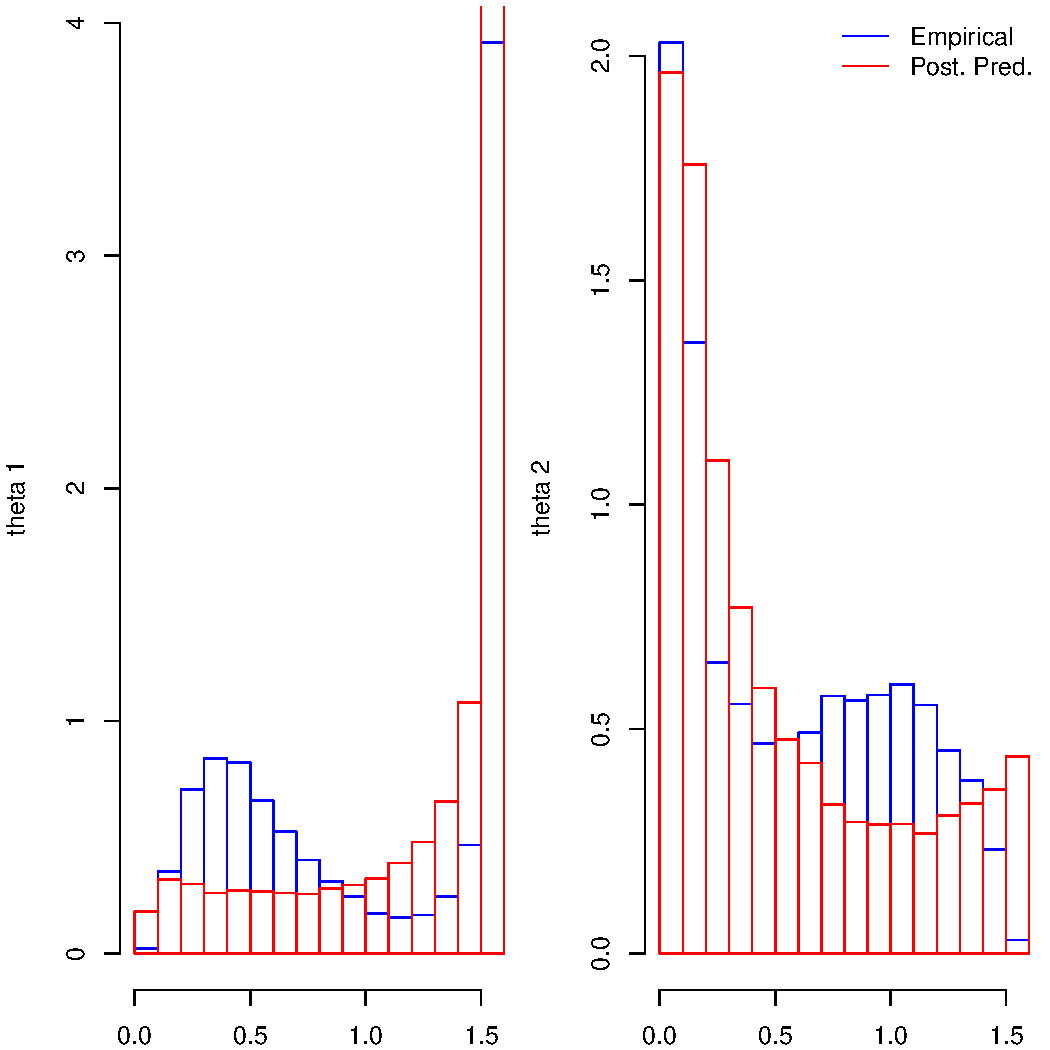
\includegraphics[width=5in]{./images/justification_for_more_complex_models}
  \caption{Histograms of Empirical vs Posterior-predictive angular data originating
            from a simulated 3-dimensional gamma dataset.}
\end{figure}

However, as flexible as it is, it alone is not sufficient for our purpose.  Supposing
  a given dataset is the result of two or more generating distributions, then using a
  a single distribution to represent this dataset becomes untenable.  In Figure~\ref{fig:vanillamix}
  we see the empirical distribution a 2-component mixture of projected gammas, plotted
  against the posterior predictive distribution of a projected gamma model fitted to
  that dataset.  As we can see, it has trouble representing the nuances of the two
  component mixture.


% EOF



\subsection{Normal model built on Probit representation of Spherical Coordinate Space}
\label{method:npprobitnorm}
The transformation in Equation~\ref{eqn:transform} provides us a mapping from $S_{2}^{d-1}$ to a
  $d-1$ dimensional cube, $[0, \pi/2]$.  Building on this transformation allows us to represent
  the data using a true $d-1$ dimensional distribution, rather than generating a latent parameter
  to induce a $d$ dimensional distribution, as we do with all the gamma based models.

A canonical choice of distribution in this space might be to further transform to $(-\infty, \infty)$
  via marginal probit or logit transformation, and represent the data as multivariate normal.  We try
  that here.   Let $W_i = \text{Probit}(2\theta_i /\pi)$--that is, scale $\theta_i$ to the unit
  interval, then conduct a probit transformation on it to result in $W_i \in (-\infty, \infty)$.
  Then we establish a multivariate normal distribution on $W$. As we are expecting data to descend
  from a mixture of distributions, we place a DP prior on the multivariate normal kernel
  distribution.  The centering distribution of the DP prior is the product of a multivariate normal
  and inverse Wishart distribution; and we place multivarite normal and inverse Wishart priors on
  these parameters.  As before, we place a gamma prior on the DP concentration parameter $\eta$.
  \begin{equation}
    \begin{aligned}
                W_i &\sim \mathcal{N}_{d-1}\left(\mu_i, \Sigma_i\right)\\
    \mu_i, \sigma_i &\sim G_i\\
                G_i &\sim \text{DP}(\eta, G_0(\mu_i,\Sigma_i\mid\mu_0,\Sigma_0))\\
                    &\hspace{1cm}G_0(\mu_i,\Sigma_i\mid\mu_0,\Sigma_0) &=
                      \mathcal{N}_{d-1}(\mu_i\mid\mu_0,\Sigma_0)\text{IW}(\Sigma\mid\nu,\psi)\\
              \mu_0 &\sim \mathcal{N}_{d-1}\left({\bf u},{\bf S}\right)\\
           \Sigma_0 &\sim \text{IW}(\nu_0,\psi_0)\\
               \eta &\sim \text{Ga}(\alpha, \beta)
    \end{aligned}
  \end{equation}
There is an advantage in that for inference on $\mu_i, \mu_0, \Sigma_i$, and $\Sigma_0$ this model
  is completely conjugate.  However, while the transformation employed in Equation~\ref{eqn:transform}
  is one to one, small deviations in different dimensions on $S_{\infty}^{d-1}$ have vastly different
  effects on the resulting transformed variables.  This induced distortion may result in an inferior
  model, when evaluating on $S_{\infty}^{d-1}$.  We will be evaluating this model as representative
  of models on the $d-1$ dimensional coordinate space, and comparing it against other models, after
  projecting back onto $S_{\infty}^{d-1}$.

Another disadvantage of this model is the need to compute $d-1$-dimensional matrix determinants
  and inversions.  If we consider that inversion is a $\mathcal{O}(n^3)$ operation, we face the real
  problem of computation time climbing astronomically as the number of dimensions grows.  We are
  currently evaluating this model on 8 and 46 dimensions, we can see that those operations on 46
  dimensions will take around 190 times longer than on 8 dimensions.  This presents a problem if we
  want to run this model in any reasonable time scale.

% EOF


\subsection{Model Comparison on the Hypercube}
It is not immediately obvious which criteria to use to judge these models and decide which best
  represents the data's generating distribution.  We have opted to use the
  \emph{posterior predictive loss} criterion of \cite{gelfand1998} and the
  \emph{energy score} criterion of \cite{gneiting2007}.  Both of these
  metrics require calculating some distance in the target space, and this section will be devoted
  to that end.  As both these metrics operate on the posterior predictive distribution for each
  observation, we will also be including a metric operating on the overall posterior predictive
  distribution, in the form of a modified Kullbeck-Liebler divergence.

\subsubsection{Posterior Predictive Loss Criterion}
The posterior predictive loss criterion, \emph{PPL} is introduced in \cite{gelfand1998}.  When we
  assume a squared error loss function, then for the $i$th observation, the posterior predictive
  loss criterion is computed as
  \begin{equation}
    \label{eq:ppl}
    D_{k}^{(i)} = \text{Var}(X_i) + \frac{k}{k + 1}\left(\text{E}[X_i] - x_i\right)^2,
  \end{equation}
  where $X_i$ is a random variable from the posterior predictive distribution for $x_i$.  The
  scalar $k$ is a weighting factor by which we arbitrarily scale the importance of goodness of fit
  relative to precision.  In our analysis, we take the limit as $k\to\infty$, and thus weight both
  parts equally.  Interpreting this criterion, a smaller $\text{Var}({\bf X}_l)$ indicates a higher
  precision, and a smaller $(\text{E}[{\bf X}_l] - {\bf x}_l)^2$  indicates a better fit.  Thus,
  smaller is better.  Note that this is defined for a univariate distribution.  As we are dealing
  with a multivariate distribution, in keeping with our spatial statistics brethren
  \makenote{find a citation where they do this}, we will be taking the posterior predictive loss
  averaged over all dimensions.  That is,
  \begin{equation}
    \label{eq:ppl2}
    D_k^{i} = \frac{1}{d}\sum_{l = 1}^{d}\left[\text{Var}(X_{il}) + \frac{k}{k+1}\left(\text{E}[X_{il}] - x_{il}\right)^2\right]
  \end{equation}
  Then we report the average $D_k$, taken over the whole dataset.

\subsubsection{Energy Score}
The energy score of Gneiting, et al\cite{gneiting2007}, is a generalization of the continuous ranked
  probability score, or \emph{crps}, defined for a multi-dimensional random variable.
  \begin{equation}
    \label{eq:es}
    \text{ES}(P,x_i) = \frac{1}{2}\text{E}_p\lVert {\bf X}_i,{\bf X}_i^{\prime}\rVert_{\Omega}^{\beta} -
                            \text{E}_p\lVert {\bf X}_i - {\bf x}_i\rVert_{\Omega}^{\beta}
  \end{equation}
  \bruno{I don't understand the first term of this expression.}
  where ${\bf X}_i^{\prime}$ is another replicate from the posterior predictive distribution
  of ${\bf x}_i$. This means, rather than relying on the first and second moments of the posterior
  predictive distribution as in the case of posterior predictive loss\cite{gelfand1998}, we are
  instead calculating pairwise distances between the observation and draws from the posterior
  predictive distribution, as well as pairwise distances between those replicates themselves.

Now here's the rub.  We are not aware of any established distance metrics developed on the
  positive orthant of the unit hypercube.  In the unit simplex, we can assume the use of
  Euclidean norm as accurately representing the distance between two points.  For any
  $\mathcal{S}_{p}^{d-1}$ space, $p > 1$, Euclidean norm is going to under-report the actual distance
  required for travel between two points.  That distortion is maximized on
  $\mathcal{S}_{\infty}^{d-1}$

The positive orthant of the unit hypercube, defined in Euclidean geometry, is that structure for
  which, in a given point on the hypercube, all dimensions of that point are between 0 and 1, and
  at least one dimension must be 1.  Developing terminology, we can consider observations for which
  the $j$th dimension is equal to 1, to be on the $j$th \emph{face}.  The intersection of the $i$th
  and $j$th face is a $d-2$ dimensional cube, and observations in this space have dimensions $i,j$
  equal to 1.

A \emph{distance} in this space is a \emph{geodesic} on this space. From geometry, we know that
  the geodesic, or shortest path between 2 points along the surface of a $d$ dimensional figure
  corresponds to at least one \emph{unfolding}, or \emph{rotation} of the $d$-dimensional
  figure into a $d-1$ dimensional space.  The appropriate term for the structure generated by this
  unfolding is a \emph{net}.  For the appropriate net, a line segment connecting the two points and
  staying within the boundaries of the net corresponds to the shortest path between those points
  \makenote{needs citation!}, and is thus a geodesic.  The length of that line segment is properly
  defines the distance required for travel between those points.

Consider a 3-dimensional cube.  Consider 2 points on this 3-dimensional cube,
  ${\bf a}_1 = (x_1,y_1,z_1)$, and ${\bf a}_2 = (x_2,y_2,z_2)$. Let's say that the two points are
  on the same face.  Then the distance between those two points, the distance one has to travel
  along the space to move from one point to the other, is calculated by Euclidean norm.  Now,
  consider two points on separate faces.  All faces are pairwise adjacent, as we have stated, so
  in order to move to the other point, we must \emph{at least} move to the intersection between the
  faces, then to the other point.  Let ${\bf a}_1$ lie on the $x$ face, and ${\bf a}_2$ lie on the
  $y$ face.  That is, ${\bf a}_1 = (1, y_1, z_1)$, ${\bf a}_2 = (x_2, 1, z_2)$.  Then traveling
  between these points we must at least pass through the intersection of faces $x,y$.  One possible
  net representation of this is unfolding the $y$ face alongside the $x$ face.  We accomplish this
  by applying a rotation and translation to $a_2$, corresponding to the following:
  \begin{equation}
    \label{eq:1drotation}
    a_2^{\prime} = \begin{bmatrix}
    1 \\
    2 \\
    0
    \end{bmatrix}
    +
    \begin{bmatrix}
    0  & 0 & 0 \\
    -1 & 0 & 0 \\
    0  & 0 & 1
    \end{bmatrix}
    \begin{bmatrix}
    x_2 \\
    1 \\
    z_2 \\
    \end{bmatrix} = \begin{bmatrix}
    1 \\
    2 - x_2 \\
    z_2
    \end{bmatrix}
  \end{equation}
  Then, if this is the appropriate net, the distance becomes
  $\lVert {\bf a}_1,{\bf a}_2\rVert = \lVert {\bf a}_1 - {\bf a}_2^{\prime}\rVert_2$ However, there
  is another possible net we must consider, travelling first through the $z$ face then to the $y$
  face.  The rotation for that becomes:
  \begin{equation}
    \label{eq:2drotation}
    a_2^{\prime} = \begin{bmatrix}
    1 \\
    2 \\
    2
    \end{bmatrix}
    +
    \begin{bmatrix}
    0 & 0 & 0  \\
    0 & 0 & -1 \\
    -1 & 0 & 0
    \end{bmatrix}
    \begin{bmatrix}
    x_2 \\
    1 \\
    z_2
    \end{bmatrix} = \begin{bmatrix}
    1 \\
    2 - z_2 \\
    2 - x_2
    \end{bmatrix}
  \end{equation}
Every successive rotation is relative to the last face.  So, as the number of dimensions grows, the
  number of possible rotations grows as well.  As we have $d$ faces, if 2 observations are on
  different faces, then there are $\sum_{j = 1}^{d-2}\binom{d-2}{j} + 1$ possible rotations to
  consider. \makenote{There are truly $d!$ possible nets, but when we consider starting and ending
  faces fixed, and that portions of the net that diverge after the ending face are irrelevant,
  we arrive at that number of rotations that we actually need consider}.  While this is not
  insurmountable, it is numerically difficult, and developing the generalized rotation strategies
  for $d$ dimensions is beyond the scope of this analysis. However, we are in luck in that all we
  need for a valid energy score is a \emph{negative definite kernel}.  This is defined as a function
  having symmetry in its arguments, $d(x_1,x_2) = d(x_2,x_1)$, and for which
  $\sum_{i =1}^n\sum_{j=1}^na_ia_jd(x_1,x_2) \leq 0$ for all positive integers n, with the
  restriction that $\sum_{i=1}^na_i = 0$.  The Euclidean norm is one example of a negative definite
  kernel.

Let's go back to that first rotation--we held that as a numerically easier analogue to our actual
  goal--the distance from the starting point, to some optimal point along the intersection between
  the starting and ending faces, to the ending point.  At that optimal point, the total distance
  travelled between starting and ending points becomes symmetric.  We can
  recognize this distance as the sum of two Euclidean norms.  That is,
  \begin{equation}
    \lVert {\bf a},{\bf b}\rVert_{H} = \lVert {\bf a}, {\bf c} \rVert_2 + \lVert {\bf c},{\bf b}\rVert_2
  \end{equation}
  If we can be assured of symmetry in the functional arguments, then the requirements for a negative
  definite kernel are trivially proved.  And from geometry\makenote{need citation on this}, we can
  assert that on a one-dimension unfolding, the line segment connecting the starting and ending
  points will travel through that optimal net.

  \bruno{This whole paragraph can be made much shorter and crispier. Introduce the problem, then mention the
         difficulty of defining an actual distance in $S_\infty^{d-1}$ and jump into the negative kernel idea,
         then write the lemma from the paper by Gneiting and Raftery, define a suitable kernel and write a
         proposition proving that it is negative definite, then comment on how you calculate it.
         BTW, I still don't understand the notation ||a,b||.}

\subsubsection{Intrinsic Energy Score}
While we have at length discussed our means of comparison between models, we have limited means of
  comparing how our model is doing relative to the data.  We introduce the
  \emph{intrinsic energy score} to offer a baseline energy score \emph{in the data}, against which
  we might compare candidate models.  This allows us to see how well our model is doing relative
  to the data, rather than just relative to other models.  We construct this using the energy score
  metric, but for any particular observation in the data, we compare that observation against all
  other observations in the data.  That is, for a given observation, treat other observations as
  replicates of that observation.  Comparing our energy score results against this value offers a
  metric of how well we are partitioning the data into separate distributions to be evaluated.

\subsection{Kullbeck Liebler Divergence}
The \emph{Kullbeck Liebler divergence} $D_{\text{KL}}$ offers a means of comparing two densities.
  It is, at its core, a logratio of the two densities, integrated over the first density.  That is,
  \begin{equation}
    \label{eqn:kld}
    D_{\text{KL}}(A,B) = \int_{x\in \Omega(A)}A(x)\log\left\frac{A(x)}{B(x)}dx
  \end{equation}
  where $\Omega(\cdot)$ indicates the support, and $A,B$ are densities.  In our case, as the
  densities are intractible, we will be estimating the densities using a numerical
  method.  There is a wealth of literature on this topic, but for reasons to be made clear, I will
  discuss two and use one.
  \bruno{You need to sharpen this explanation and possibly include a formula.}

Parzen \cite{parzen1962} offers a method of density estimation involving setting a window with
  radius $\sigma$ around a point, and counting observations within that window.  The number of
  observations within the window, divided by the total number of observations within the dataset,
  and the area of the window provides an estimate of the density at that point. This is highly
  dependent upon the choice of window radius $\sigma$, but importantly for our purpose, the
  \emph{area} of the window on $S_{\infty}^{d-1}$ is not well defined.  Consider $S_{\infty}^{2}$,
  the surface of the positive orthant of the cube.  Now imagine a circle.  Imagine plastering that
  circle on different points of the cube.  If the circle is entirely contained on one face of the
  cube, it can spread out and exhibit its full area.  If it crosses between 2 faces, it can still
  exhibit its full area. But if we place that circle with its center at $(1,1,1)$, then plaster down
  the sides, we are left with 1/4 of the circle unable to be pasted down.  That is, The circle at
  that point has an area of only $\frac{3}{4}\pi r^2$ whereas a circle of radius $r$ not
  intersecting that point will have an area of $\pi r^2$.  In higher dimensions, this relationship
  becomes more murky.

Even outside of our specific geometry, the Parzen method suffers another issue--the curse of
  dimensionality.  \cite{boltz2009} shows, for finite sample size, that as the number of dimensions
  increases, the probability of observations falling into the window on the other dataset decreases.
  Effectively, the quality of density estimation goes down as dimensionality goes up.

An alternative to this method that we will use is based on distance between observations from the
  empirical and posterior predictive distributions.  Similar to the Parzen method, we're working
  with samples from the distribution, but instead of establishing a window of some width, we're
  using distance from the target observation to its $k$ nearest neighbors in the dataset.
  From hence, we get the name \emph{KNN Based KL Divergence}.  The \emph{FNN} package in R implements
  a Euclidean distance based version of this approach.  As we operate on the hypersphere, we again
  recognize that the Euclidean distance metric is not appropriate, delivering results strongly
  biased downwards.  Our one-rotation norm method described previously is employed here as a
  distance.  We recognize that the one-rotation norm is on average biased slightly longer as
  compared to a proper geodesic, but it is closer to truth than any other distance metric we are
  aware of.  To that end, we employ it as the pairwise distance measure required by KNN for this KNN
  based KL divergence.  We employ the formula of Boltz et al \cite{boltz2009}, as
  \begin{equation}
    \label{eqn:knnkld}
    D_{\text{KL}}^{(k)}(A,B) = \log\frac{n(B)}{n(A)} + c(A) \left[\rho_A^{(k)}(B)
                                                                      - \rho_A^{(k)}(A)\right]
  \end{equation}
  where $\rho_A(\cdot)$ denotes the average log-distance for observations in $A$ to their $k$th
  nearest observation in $\cdot$.  Boltz et al acknowledge that their method is biased, does not
  integrate to 1, but its disadvantages in bias as compared to the Parzen windowing method are less
  apparent at higher dimensions, where the windowing method's weakness to dimensionality tends to
  rise.  As we regard this as a numerical approximation, we offer this metric in the spirit of
  complementary evidence, rather than an authority, or oracle, to show us the way.































% EOF


\subsection{Spatial Threshold Modeling}
Following the work of \cite{ferreira2014}, any of the above methods can be
  extended to the spatial domain by modification of the marginalization process.
  Assume a spatial process $X({\bf s})$, ${\bf s}\in {\bf S}$.  Then take the
  transformation
\begin{equation}
  \label{eqn:spatial}
  Z({\bf s}) = \left(1 + \gamma({\bf s})\frac{X({\bf s}) - b_t({\bf s})}{a_t({\bf s})}\right)_{+}^{1/{\gamma({\bf s})}}
\end{equation}
  where $b_t({\bf s})$ is a function corresponding to a high threshold at location
  ${\bf s}$, analogous to the role $b_t$ played previously. $a_t({\bf s})$
  corresponds to a scaling function, and $\gamma({\bf s})$ an extremal value index
  function.

% EOF


\section{Model Comparison on the Hypersphere}
It is not immediately obvious what criteria to use to judge these models and decide which best
  represents the data's generating distribution.  As the task resides on $\mathcal{S}_{\infty}^{d-1}$,
  our options are somewhat limited in terms of what model criteria we can use.  Because of the aforementioned
  difficulty in evaluating a density directly in this space, we choose to use model evaluation
  criteria that can operate on samples from the posterior predictive distribution.  For this reason,
  we have opted to use the \emph{posterior predictive loss} criterion of \cite{gelfand1998} and the
  \emph{energy score} criterion of \cite{gneiting2007}.  Both of these metrics require calculating
  some distance in the target space, and this section will be devoted to that end.  As both these
  metrics operate on the posterior predictive distribution for each observation, we will also be
  including a metric operating on the overall posterior predictive distribution, in the form of a
  modified Kullbeck-Liebler divergence.

\subsection{Posterior Predictive Loss Criterion}
The posterior predictive loss criterion, \emph{PPL} is introduced in \cite{gelfand1998}.  When we
  assume a squared error loss function, then for the $i$th observation, the posterior predictive
  loss criterion is computed as
  \begin{equation}
    \label{eq:ppl}
    D_{k}^{(i)} = \text{Var}(X_i) + \frac{k}{k + 1}\left(\text{E}[X_i] - x_i\right)^2,
  \end{equation}
  where $X_i$ is a random variable from the posterior predictive distribution for $x_i$.  The
  scalar $k$ is a weighting factor by which we arbitrarily scale the importance of goodness of fit
  relative to precision.  In our analysis, we take the limit as $k\to\infty$, and thus weight both
  parts equally.  Interpreting this criterion, a smaller $\text{Var}({\bf X}_l)$ indicates a higher
  precision, and a smaller $(\text{E}[{\bf X}_l] - {\bf x}_l)^2$  indicates a better fit.  Thus,
  smaller is better.  Note that this is defined for a univariate distribution.  As we are dealing
  with a multivariate distribution, in keeping with our spatial statistics brethren
  \makenote{find a citation where they do this}, we will be taking the posterior predictive loss
  summed over all dimensions.  That is,
  \begin{equation}
    \label{eq:ppl2}
    D_k^{(i)} = \frac{1}{d}\sum_{l = 1}^{d}\left[\text{Var}(X_{il}) + \frac{k}{k+1}\left(\text{E}[X_{il}] - x_{il}\right)^2\right]
  \end{equation}
  Then we report the average $D_k$, taken over all $i$.

\subsection{Energy Score}
The energy score of Gneiting, et al\cite{gneiting2007}, is a generalization of the continuous ranked
  probability score, or \emph{crps}, defined for a multi-dimensional random variable.
  \begin{equation}
    \label{eq:es}
    \text{ES}(P,x_i) = \frac{1}{2}\text{E}_p g(\bm{X}_i,\bm{X}_i^{\prime}) - \text{E}_p g(\bm{X}_i, \bm{x}_i)
  \end{equation}
  where $g(\cdot)$ identifies a negative definite kernel, and $\bm{X}_i^{\prime}$ represents another
  replicate from the posterior predictive distribution of $\bm{x}_i$. The negative definite kernel
  most often used is Euclidean distance.  However,on $\mathcal{S}_p^{d-1}$ for $p > 1$, Euclidean
  distance can under-report the actual distance required for travel between two points. That distortion
  is maximized on $\mathcal{S}_{\infty}^{d-1}$.

\subsection{Distance on the positive orthant of the Hypercube}
  \label{subsec:distance}
The positive orthant of the unit hypercube, defined in Euclidean geometry, is that structure for
  which, in a given point on the hypercube, all dimensions of that point are between 0 and 1, and
  at least one dimension must be 1.  Developing terminology, we can consider observations for which
  the $j$th dimension is equal to 1, to be on the $j$th \emph{face}.  The intersection of the $i$th
  and $j$th face is a $d-2$ dimensional cube, and observations in this space have dimensions $i,j$
  equal to 1.

A \emph{distance} in this space is a \emph{geodesic} on this space. From geometry, we know that
  the geodesic, or shortest path between 2 points along the surface of a $d$ dimensional figure
  corresponds to at least one \emph{unfolding}, or \emph{rotation} of the $d$-dimensional
  figure into a $d-1$ dimensional space.  The appropriate term for the structure generated by this
  unfolding is a \emph{net}.  For the appropriate net, a line segment connecting the two points and
  staying within the boundaries of the net corresponds to the shortest path between those points
  \makenote{needs citation!}, and is thus a geodesic.  The length of that line segment is properly
  defines the distance required for travel between those points.

Consider a 3-dimensional cube.  Consider 2 points on this 3-dimensional cube,
  ${\bf a}_1 = (x_1,y_1,z_1)$, and ${\bf a}_2 = (x_2,y_2,z_2)$. Let's say that the two points are
  on the same face.  Then the distance between those two points, the distance one has to travel
  along the space to move from one point to the other, is calculated by Euclidean norm.  Now,
  consider two points on separate faces.  All faces are pairwise adjacent, as we have stated, so
  in order to move to the other point, we must \emph{at least} move to the intersection between the
  faces, then to the other point.  Let ${\bf a}_1$ lie on the $x$ face, and ${\bf a}_2$ lie on the
  $y$ face.  That is, ${\bf a}_1 = (1, y_1, z_1)$, ${\bf a}_2 = (x_2, 1, z_2)$.  Then traveling
  between these points we must at least pass through the intersection of faces $x,y$.  One possible
  net representation of this is unfolding the $y$ face alongside the $x$ face.  We accomplish this
  by applying a rotation and translation to $a_2$, corresponding to the following:
  \begin{equation}
    \label{eq:1drotation}
    a_2^{\prime} = \begin{bmatrix}
    1 \\
    2 \\
    0
    \end{bmatrix}
    +
    \begin{bmatrix}
    0  & 0 & 0 \\
    -1 & 0 & 0 \\
    0  & 0 & 1
    \end{bmatrix}
    \begin{bmatrix}
    x_2 \\
    1 \\
    z_2 \\
    \end{bmatrix} = \begin{bmatrix}
    1 \\
    2 - x_2 \\
    z_2
    \end{bmatrix}
  \end{equation}
  Then, if this is the appropriate net, the distance becomes
  $\lVert {\bf a}_1,{\bf a}_2\rVert = \lVert {\bf a}_1 - {\bf a}_2^{\prime}\rVert_2$ However, there
  is another possible net we must consider, travelling first through the $z$ face then to the $y$
  face.  The rotation for that becomes:
  \begin{equation}
    \label{eq:2drotation}
    a_2^{\prime} = \begin{bmatrix}
    1 \\
    2 \\
    2
    \end{bmatrix}
    +
    \begin{bmatrix}
    0 & 0 & 0  \\
    0 & 0 & -1 \\
    -1 & 0 & 0
    \end{bmatrix}
    \begin{bmatrix}
    x_2 \\
    1 \\
    z_2
    \end{bmatrix} = \begin{bmatrix}
    1 \\
    2 - z_2 \\
    2 - x_2
    \end{bmatrix}
  \end{equation}
Every successive rotation is relative to the last face.  So, as the number of dimensions grows, the
  number of possible rotations grows as well.  As we have $d$ faces, if 2 observations are on
  different faces, then there are $\sum_{j = 1}^{d-2}\binom{d-2}{j} + 1$ possible rotations to
  consider. \footnote{There are truly $d!$ possible nets, but when we consider starting and ending
  faces fixed, and that portions of the net that diverge after the ending face are irrelevant,
  we arrive at that number of rotations that we need consider}.  While this is not
  insurmountable, it is numerically difficult, and developing the generalized rotation strategies
  for $d$ dimensions is beyond the scope of this analysis. However, we are in luck in that all we
  need for a valid energy score is a \emph{negative definite kernel}.  This is defined as a function
  having symmetry in its arguments, $d(x_1,x_2) = d(x_2,x_1)$, and for which
  $\sum_{i =1}^n\sum_{j=1}^na_ia_jd(x_1,x_2) \leq 0$ for all positive integers n, with the
  restriction that $\sum_{i=1}^na_i = 0$.  The Euclidean norm is one example of a negative definite
  kernel.

Let's go back to that first rotation--we held that as a numerically easier analogue to our actual
  goal--the distance from the starting point, to some optimal point along the intersection between
  the starting and ending faces, to the ending point.  At that optimal point, the total distance
  travelled between starting and ending points becomes symmetric.  We can
  recognize this distance as the sum of two Euclidean norms.  That is,
  \begin{equation}
    \lVert {\bf a},{\bf b}\rVert_{H} = \lVert {\bf a}, {\bf c} \rVert_2 + \lVert {\bf c},{\bf b}\rVert_2
  \end{equation}
  If we can be assured of symmetry in the functional arguments, then the requirements for a negative
  definite kernel are trivially proved.  And from geometry\makenote{need citation on this}, we can
  assert that on a one-dimension unfolding, the line segment connecting the starting and ending
  points will travel through that optimal net.

  \bruno{This whole paragraph can be made much shorter and crispier. Introduce the problem, then mention the
         difficulty of defining an actual distance in $S_\infty^{d-1}$ and jump into the negative kernel idea,
         then write the lemma from the paper by Gneiting and Raftery, define a suitable kernel and write a
         proposition proving that it is negative definite, then comment on how you calculate it.
         BTW, I still don't understand the notation ||a,b||.}

% \subsubsection{Intrinsic Energy Score}
% While we have at length discussed our means of comparison between models, we have limited means of
%   comparing how our model is doing relative to the data.  We introduce the
%   \emph{intrinsic energy score} to offer a baseline energy score \emph{in the data}, against which
%   we might compare candidate models.  This allows us to see how well our model is doing relative
%   to the data, rather than just relative to other models.  We construct this using the energy score
%   metric, but for any particular observation in the data, we compare that observation against all
%   other observations in the data.  That is, for a given observation, treat other observations as
%   replicates of that observation.  Comparing our energy score results against this value offers a
%   metric of how well we are partitioning the data into separate distributions to be evaluated.

\subsection{Kullbeck Liebler Divergence}
The \emph{Kullbeck Liebler divergence} $D_{\text{KL}}$ offers a means of comparing two densities.
  It is, at its core, a log-ratio of the two densities, integrated over the first density.  That is,
  \begin{equation}
    \label{eqn:kld}
    D_{\text{KL}}(A,B) = \int_{x\in \Omega(A)}A(x)\log\left(\frac{A(x)}{B(x)}\right)dx
  \end{equation}
  where $\Omega(\cdot)$ indicates the support, and $A,B$ are densities.  As the KL divergence is not
  symmetric, it is not referred to as a \emph{distance} between densities, but it is often employed
  as a means of comparison.  In our case, as the densities are intractible, we will be computing an
  estimate of the KL divergence using a numerical method of estimating the density.

Parzen \cite{parzen1962} offers a method of density estimation involving setting a window with
  radius $\sigma$ around a point, and counting observations within that window.  The number of
  observations within the window, divided by the total number of observations within the dataset,
  and the area of the window provides an estimate of the density at that point. This is highly
  dependent upon the choice of window radius $\sigma$.  Furthermore, the Parzen method suffers
  another issue--the curse of dimensionality.  \cite{boltz2009} shows, for finite sample size, that
  as the number of dimensions increases, the probability of observations falling into the window on
  the other dataset decreases. Effectively, the quality of density estimation goes down as
  dimensionality goes up.

An alternative to this method that we will use is based on distance between observations from the
  empirical and posterior predictive distributions.  Similar to the Parzen method, we're working
  with samples from the distribution, but instead of establishing a window of some width, we are
  using distance from the target observation to its $k$th nearest neighbor in the dataset.
  From hence we get the name \emph{KNN Based KL Divergence}.  As we operate on the hypersphere,
  we again recognize that the Euclidean distance metric is not appropriate, delivering results strongly
  biased downwards.  Our one-rotation kernel method described previously is employed here as a
  distance.  We recognize that the one-rotation norm is on average biased slightly longer as
  compared to a proper geodesic, but it is closer to truth than any other distance metric we are
  aware of.  To that end, we employ it as the pairwise distance measure required by KNN for this KNN
  based KL divergence.  We employ the formula of Boltz et al \cite{boltz2009}, as
  \begin{equation}
    \label{eqn:knnkld}
    D_{\text{KL}}^{(k)}(A,B) = \log\frac{n(B)}{n(A)} + c(A) \left[\rho_A^{(k)}(B)
                                                                      - \rho_A^{(k)}(A)\right]
  \end{equation}
  where $\rho_A(\cdot)$ denotes the average log-distance for observations in $A$ to their $k$th
  nearest observation in $\cdot$.  Boltz et al acknowledge that their method is biased, does not
  integrate to 1, but its disadvantages in bias as compared to the Parzen windowing method are less
  apparent at higher dimensions, where the windowing method's weakness to dimensionality tends to
  rise.  As we regard this as a numerical approximation, we offer this metric in the spirit of
  complementary evidence, rather than an authority, or oracle, to show us the way.































% EOF


% results.tex

\section{Results}

% results_simulation.tex
\subsection{Simulation}









% EOF


% results.tex
\subsection{Integrated Vapor Transport}
We use data from the integrated water vapor transport (\emph{IVT}) model\makenote{needs citation}
  of atmospheric rivers as a means of testing these models.  An atmospheric river is a meteorological
  event of local concentration of water vapor in the atmosphere that moves with wind patterns.
  Understanding dependence among extreme events in atmospheric rivers \makenote{finish thought}.

Fitting our models to this data requires some pre-processing.  The marginal distributions of the
  IVT data appear naturally log-normal, which falls into the domain of attraction of a Gumbel
  distribution.  Given that, we can apply a high threshold, and exceedances over that threshold can
  be modelled as Generalized Pareto.  Our model begins with that assessment.  As estimating
  the Pareto parameters is not yet our focus in this analysis, we choose to apply the threshold
  using the empirical CDF.  That is, for a given $t$, let $b_{tl} = \hat{F}_l^{-1}(1 - t^{-1})$.  For
  this analysis, we set $t = 20$, indicating the marginal $95$ percentile.  The other parameters of the
  generalized Pareto--the scale parameter $\alpha_{tl}$ and the extremal index $\chi_l$--are set via
  maximum likelihood.  A fully Bayesian model formulation will allow their varying within a
  distribution, but such a model formulation will not be conducive to fitting by Markov-chain Monte
  Carlo methods.

After the thresholding and maximum likelihood estimation of the parameters of the Pareto, we scale
  the data to the standard multivariate Pareto.  Dividing each standardized observation by its
  $\mathcal{L}_{\infty}$ norm, we project the standardized data onto the hypercube.  Data in sequence
  represents observations in time, and these are heavily correlated.  As such, we choose to
  \emph{decluster} the observations, such that, by observing a sequence of observations ${\bf z}$
  for which $\inorm{z_i} > 1$ for each observation in sequence, we keep only the observation with
  the maximum observed $\mathcal{L}_{\infty}$ norm.  The complete procedure is outlined in
  Algorithm~\ref{algo:processing}.

\begin{algorithm}
  \label{algo:processing}
  \KwResult{${\bf r} : r_i \sim \text{Pareto}(1)$, ${\bf v} \in \mathcal{S}_{\infty}^{d-1}$}
  \For{$l = 1,ldots,d$}{
    Set $b_{tl} = \hat{F}_l^{-1}\left(1 - \frac{1}{t}\right)$.\\
    With ${\bf x}_l > b_{tl}$, fit $a_{tl}$, $\chi_l$ via MLE according to generalized Pareto likelihood.\\
    }
  \For{$i = 1,\ldots,n$}{
    Define $z_{il} = \left(1 + \xi_l\frac{x_{il} - b_{t,l}}{a_{t,l}}\right)_{+}^{1/\xi_l}$\\
    Define $r_i = \pnorm{{\bf z}_i}{\infty}$, ${\bf V}_i = \frac{{\bf z}_i}{\pnorm{{\bf z}_i}}$\\
    }
  Subset ${\bf r},{\bf v}$ such that $r_i \geq 1$ for all $r_i\in {\bf r}$.\\
  \If{declustering}{
    \For{$i = 1,\ldots,n$}{
      If $r_i \geq 1$ and $r_{i-1} \geq 1$, drop the lesser (and associated $v_i$) from dataset.
    }
\end{algorithm}

Post-standardization, we assume the radial component to follow a standard Pareto distribution.  The
  subject of this paper is a parametric representation of the angular component ${\bf v}$, to which
  we fit the models presented.  We then generate samples from the posterior predictive
  distributions--both overall, for use with the KL divergence metric, and conditioned on individual
  observations, for use with the posterior predictive loss and energy score metrics.

We have, at our disposal, two datasets from the IVT model.  One records data from 8 grid cells,
  covering generally the coast of California.  The other, with a higher resolution, records data
  from 46 grid cells covering the same area.  We fit our models to both datasets.

\begin{table}[h]
  \label{tab:dev}
  
\begin{tabular}{cccccccc}
\toprule
\multicolumn{4}{c}{ } & \multicolumn{2}{c}{dim = 8} & \multicolumn{2}{c}{dim = 46} \\
\cmidrule(l{3pt}r{3pt}){5-6} \cmidrule(l{3pt}r{3pt}){7-8}
Model & Norm & Mix & Prior & PPL & ES & PPL & ES\\
\midrule
Gamma & L1 &  &  & 1.816 & 0.840 & 6.616 & 1.632\\
Gamma & L1 & DP & Gamma & 0.795 & 0.422 & 4.514 & 1.258\\
Gamma & L1 & DP & LogNormal & 0.386 & 0.277 & 2.396 & 0.822\\
Gamma & L1 & M & Gamma & 0.525 & 0.349 & 3.029 & 0.975\\
Gamma & L1 & M & LogNormal & 0.638 & 0.371 & 3.779 & 1.105\\
\addlinespace
Gamma & L2 &  &  & 1.816 & 0.840 & 6.616 & 1.633\\
Gamma & L2 & DP & Gamma & 0.775 & 0.408 & 5.573 & 1.480\\
Gamma & L2 & DP & LogNormal & 0.370 & 0.265 & 2.424 & 0.835\\
Gamma & L2 & M & Gamma & 0.579 & 0.366 & 2.826 & 0.935\\
Gamma & L2 & M & LogNormal & 0.577 & 0.349 & 5.165 & 1.396\\
\addlinespace
Gamma & Linf & DP & Gamma & 0.845 & 0.444 & 6.348 & 1.651\\
Gamma & Linf & DP & LogNormal & 0.384 & 0.278 & 2.376 & 0.823\\
Gamma & Linf & M & Gamma & 0.538 & 0.352 & 3.067 & 0.986\\
Gamma & Linf & M & LogNormal & 0.584 & 0.359 & 3.785 & 1.129\\
Probit Normal &  & DP & Normal & 0.842 & 0.445 & 8.021 & 1.611\\
\addlinespace
Res. Gamma & L1 &  &  & 1.820 & 0.818 & 6.774 & 1.546\\
Res. Gamma & L1 & DP & Gamma & 0.200 & 0.173 & 2.427 & 0.834\\
Res. Gamma & L1 & DP & LogNormal & 0.230 & 0.193 & 1.642 & 0.656\\
Res. Gamma & L1 & M & Gamma & 0.214 & 0.190 & 1.411 & 0.620\\
Res. Gamma & L1 & M & LogNormal & 0.222 & 0.191 & 1.445 & 0.616\\
\addlinespace
Res. Gamma & L2 &  &  & 1.820 & 0.819 & 6.777 & 1.546\\
Res. Gamma & L2 & DP & Gamma & 0.202 & 0.176 & 2.037 & 0.772\\
Res. Gamma & L2 & DP & LogNormal & 0.273 & 0.210 & 1.652 & 0.643\\
Res. Gamma & L2 & M & Gamma & 0.217 & 0.189 & 1.794 & 0.704\\
Res. Gamma & L2 & M & LogNormal & 0.248 & 0.201 & 1.270 & 0.528\\
\addlinespace
Res. Gamma & Linf & DP & Gamma & 0.191 & 0.168 & 2.019 & 0.776\\
Res. Gamma & Linf & DP & LogNormal & 0.228 & 0.191 & 1.458 & 0.589\\
Res. Gamma & Linf & M & Gamma & 0.219 & 0.191 & 1.554 & 0.664\\
Res. Gamma & Linf & M & LogNormal & 0.222 & 0.189 & 1.266 & 0.530\\
\bottomrule
\end{tabular}

\end{table}

As is visible from Table~\ref{tab:dev}, we see a strong preference for the mixture models as
  compared to the vanilla models both in posterior predictive loss and energy score.  As these
  measure model performance conditional on the observed data's posterior mixture component flags,
  it would likely be the case that a mixture model is preferred as compared to a single model.  We
  also employ the KL divergence metric to look for differences in kernel density.

That said, there is much we can glean from this table.  The normal model, which we developed after
  having cast the data from $S_{\infty}^{d-1}$ to the $d-1$ cube $[0,\pi/2]^{d-1}$ via spherical
  coordinate transformation, then scaled via probit transformation to $(-\infty,\infty)$, was not
  competitive when we transform samples from its posterior predictive distribution back onto
  $S_{\infty}^{d-1}$. The spherical coordinate transformation induces a high degree of dependence
  between dimensions, so it is difficult to think of the geometry of that space as orthogonal.
  Never the less, fitting a normal model in that space assumes something like orthogonality, which
  obviously doesn't hold.  The resulting low model performance in the normal model is likely a
  result of this distortion.

Another inference to learn from this table is the generally better results of the restricted Gamma
  models--Dirichlet, projected restricted Gamma--as compared to the Gamma models that allow for a
  varying rate parameter--generalized Dirichlet and projected Gamma.  Note that regardless of what
  prior was used for the shape parameter, we always assumed a Gamma prior for the rate parameter if
  we allowed it to vary.  In one model formulation, we attempted a multivariate log-normal prior that
  covered both the rate and shape parameters, but this overall resulted in worse model performance
  even comparing to our current results.

It is no surprise that Dirichlet process models are generally preferred as compared to the finite
  mixture models.  Properly tuned, finite mixture models will likely only do \emph{as well} as the
  Dirichlet process mixture model when their number of extant model components are in rough
  agreement.  The Dirichlet process just allows us to bypass to some extent that tuning process.
  That said, for a given performance, the finite mixture model would be preferred, as much of the
  model sampling can be accomplished in parallel.

The final, and most important, revelation this table contains concerns relative model performance
  between the incarnations of the restricted Gamma model.  Given the mixture method, the Dirichlet
  and projected restricted Gamma model are effectively the same model, just built on a different
  projection of the original data.  And indeed, on the 8 dimensional data, the model performance is
  comparable.  But on the higher dimensional data, we see model performance favor the model built on
  $S_{2}^{d-1}$ rather than $S_1^{d-1}$, the simplex.  That difference in model performance is of
  interest.

\begin{figure}[h]
  \centering
  \label{fig:knnkl}
  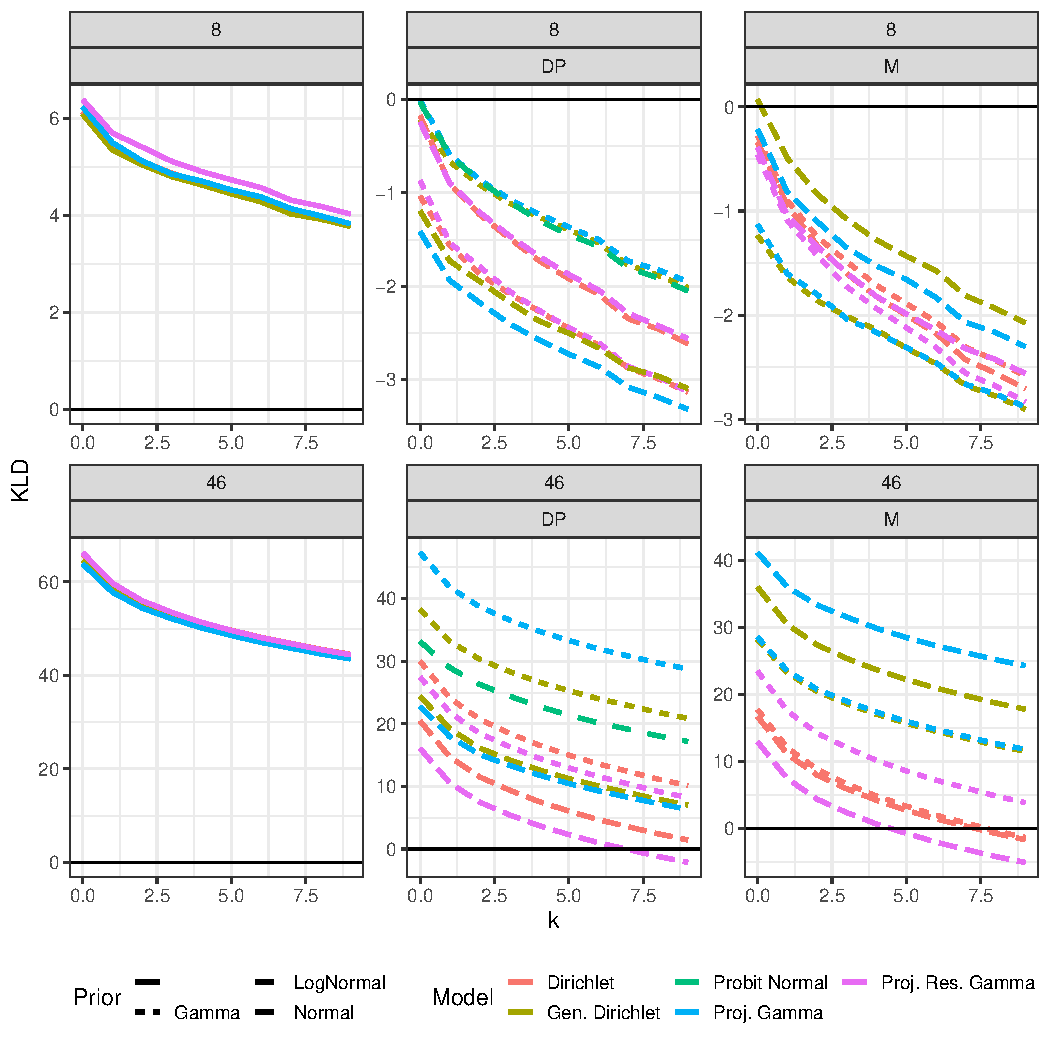
\includegraphics[width = 5in]{./images/kl_divergence_curves}
  \caption{KL Divergence Curves calculated through the KNN-KL Metric, evaluated between the empirical
  dataset and posterior predictive datasets of various models.  The top row corresponds to the
  8-dimensional data, while the bottom row the 46.  The left column corresponds to the vanilla models
  with no mixture method; the middle column a Dirichlet process prior, and the right column a finite
  mixture model.}
\end{figure}

Interpreting the KL divergence curves in Figure~\ref{fig:knnkl}, KL divergence at its core is a
  log-ratio of densities.  We would prefer, all else being equal, a KL divergence near 0.
  Interpreting this particular divergence metric, a KL divergence less than 0 means on average,
  that the $k$th closest sample from the posterior predictive dataset is closer to the observation
  than the $k$th closest sample from the empirical dataset.  There is a logged ratio of sample sizes
  to account for differences in cardinality between the empirical dataset and posterior predictive.

From this, we would interpret the \emph{best} model as that model which remains closest to the
  horizontal line at $0$.  For the 8-dimension model, this means the generalized Dirichlet and
  projected Gamma models, the unrestricted Gamma based models, seem to perform the best.   This is
  in stark contrast to our inference from the earlier posterior predictive loss and energy score
  criterions, which sharply favored the restricted Gamma models.  However, as dimensionality
  increases, we see that the restricted Gamma models again become favored, indicating that the
  greater flexibility of the unrestricted Gamma models becomes burdensome to fit in a
  high-dimensional case.



% EOF


% EOF


\section{Applications of EVT Analysis}
\label{ref:applications}
Representing the angular component of the Pareto process with a (semi) parametric distribution grants
  us opportunities in posterior analysis.
%
% \subsection{Face Probabilities}
% One of the simplest inferences we can make from this model would be the probability of a particular
%   dimension being max--the probability of falling on a particular face.  This provides us an
%   understanding on which dimensions are more likely to be extreme.
%   \begin{equation}
%     \text{P}\left(Z_l = \max_{i}Z_i\right) = \text{P}\left(V_l = 1\right) = \text{E}\left[1_{V_l = 1}\right]
%   \end{equation}
%   Even in the gamma case, this is difficult to calculate directly. Were we to find an analytic form
%   of this quantity, we could approach the problem of establishing a density on $\mathcal{S}_{\infty}^{d-1}$
%   in the manner outlined in Eqn.~\ref{eqn:mixconddensity}.  However, we can calculate this via
%   Monte Carlo integration; in much the same manner as we will calculate the other inferences in this
%   section.

\subsection{Pairwise Extremal Dependence Coefficients}
A summary measure of extremal dependence between dimensions can be offered by the extremal dependence
  coefficient.  This can be thought of as something like a correlation coefficient for extreme
  observations.  For a random variable $\bm{Z}$, which has been standardized such that the marginal
  distributions are common between dimensions, it is defined as
  \begin{equation}
    \chi_{kl} = \lim\limits_{u\to\infty}\text{P}\left(Z_k > u\mid Z_l > u\right).
  \end{equation}
  The value $\chi_{kl} \in [0,1]$.  When $\chi_{kl}$ approaches 1, that indicates complete dependence;
  the variables are linked, in much the same manner as if a correlation coefficient approaches 1.
  When $\chi_{kl}$ is greater than 0, $X_k$ and $X_l$ are considered asymptotically dependent.  For
  a $\bm{Z}$ distributed by a Pareto process, \cite{warner2018} transform $Z$ to the unit square to
  re-express this quantity,
  \begin{equation}
    \label{eqn:extdepcoef}
    \chi_{kl} = \text{E}\left[\frac{V_k}{\text{E}(V_k)}\wedge\frac{V_l}{\text{E}(V_l)}\right]
  \end{equation}
  for $V_k,V_l \in [0,1]$ \bruno{Please remind readers that $V = Z/||Z||\infty$}.  This calculation is wholely dependent on the angular component, as radial
  measure is independent of angular measure.  Important to note, however, is that complete asymptotic
  independence, where $\chi_{kl} := 0$, can not be described under a Pareto process based model.

  \begin{figure}[ht!]
    \centering
    \label{fig:chi_ij}
    \begin{minipage}{.49\textwidth}
      \centering
      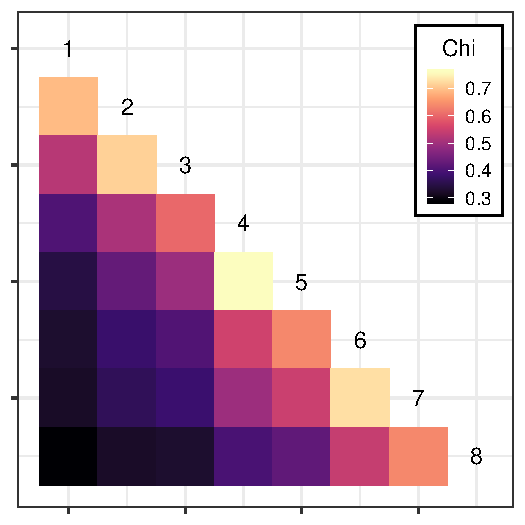
\includegraphics[width=0.99\linewidth]{./images/chi_ij_8}
    \end{minipage}
    \begin{minipage}{.49\textwidth}
      \centering
      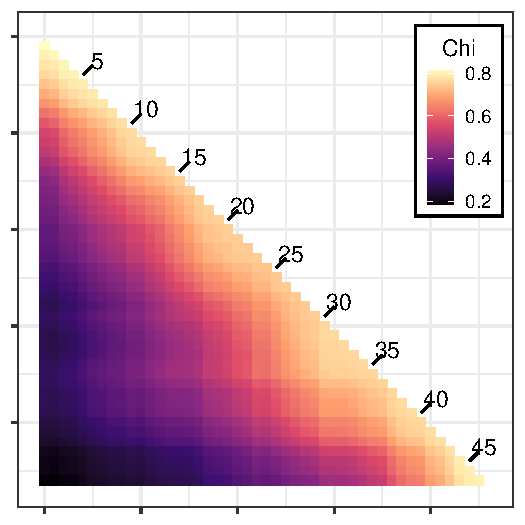
\includegraphics[width=0.99\linewidth]{./images/chi_ij_46}
    \end{minipage}
    \caption{Pairwise extremal dependence coefficients for IVT data, computed from fitted DP mixture
      of projected restricted gamma model.  The left corresponds to the 8-cell data, the right the
      47-cell data.}
  \end{figure}

Figure~\ref{fig:chi_ij} plots the pairwise extremal dependence coefficients for the IVT data, in 8
  cells (left) and 47 cells (right), computed fom a fitted DP mixture of projected restricted gammas.
  We see a higher extremal dependence between neighboring columns which is not unexpected, as
  neighboring columns correspond to neighboring cells.  We recognize that pairwise asymptotic dependence
  coefficients tell a limited story, as a particular dependence may structure may include more than
  two columns.   We can, however, glean some information from the patterns that emerge in two dimensions.
  On the 8-cell data, we see a stronger association between cells 5-8, indicating a greater
  dependence among these cells.  On the 47 cell data, we see at least 3 groupings of columns,
  indicating greater asymptotic dependence among these groups.

\subsection{Conditional Survival Curves}
Another interesting inference we can make from a fitted model is a conditional survival curve.
  Following rules of conditional probability, we can develop survival curves based on
  threshold exceedences. For ${\bf Z} = (Z_1,\ldots,Z_d)$ following a $d$-variate Pareto distribution,
  In 1 dimension, the conditional survival function can be developed as
  \begin{equation}
    \label{eqn:condsurv1d}
    \text{P}\left(Z_l > z_l\mid {\bf Z}_{-(l)} > {\bf z}_{-(l)}\right) =
      \frac{\text{P}\left(\cap_{k = 1}^d Z_k > z_k\right)}{\text{P}\left(\cap_{k \neq l} Z_k > z_k\right)}.
  \end{equation}
  Let $R = \pnorm{{\bf Z}}{\infty}$, ${\bf V} = \frac{{\bf Z}}{R}$, such that ${\bf V}\in \mathcal{S}_{\infty}^{d-1}$.
  For evaluating these probabilities, recall that ${\bf Z} = R{\bf V}$.  Then,
  \begin{equation}
    \text{P}\left(\cap_{k = 1}^d Z_k > z_k\right) = \text{P}\left(\cap_{k = 1}^d RV_k > z_k\right)
  \end{equation}
  Also, for standard Pareto, recall that $\text{P}(R > r) = 1\wedge\frac{1}{r}$.  Then,
  \begin{equation}
    \text{P}\left(\bigcap_{k = 1}^d R > \frac{z_k}{v_k}\right) =
      \text{P}\left(R  > \bigvee_{k=1}^d\frac{z_k}{V_k}\right) =
      \text{E}\left[1 \bigwedge \left(\bigvee_{k = 1}^d\frac{z_k}{V_k}\right)^{-1}\right].
  \end{equation}
  As $V_k \in [0,1]$, and given our interest in the tail of the distribution, we can assume $z_k > 1$,
  therefore $\frac{z_k}{V_k} > 1$.  We thus arrive at
  \begin{equation}
    \text{P}\left(\cap_{k = 1}^dZ_k > z_k\right) = \text{E}\left(\wedge_{k = 1}^d\frac{V_i}{z_i}\right).
  \end{equation}
  We employ a similar calculation in the denominator, yielding
  \begin{equation}
    \label{eqn:condsurv1df}
    \text{P}\left(Z_l > z_l\mid {\bf Z}_{\neg(l)} > {\bf z}_{\neg(l)}\right) =
      \frac{\text{E}\left[\wedge_{k = 1}^d \frac{V_k}{z_k}\right]}{\text{E}\left[\bigwedge_{k \neq l}\frac{V_k}{z_k}\right]}.
  \end{equation}
  Figure~\ref{fig:condsurv1d} displays this conditional survival function for the 8 cell data. For each
  cell, the survival function is computed given all other cells are at or above their $90$th marginal
  percentile.

\begin{figure}[h]
  \label{fig:condsurv1d}
  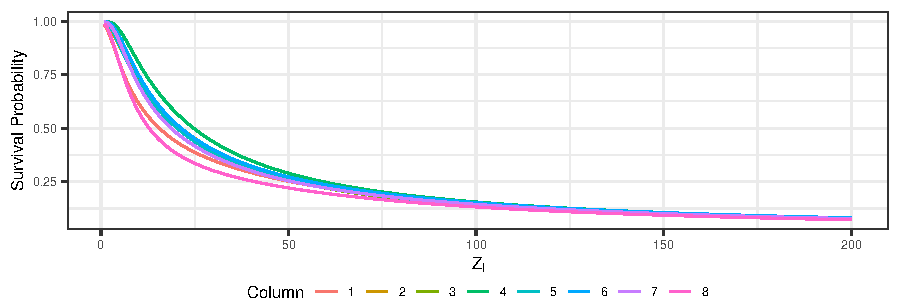
\includegraphics{./images/condsurv_1d}
  \caption{
    Single-variable conditional survival function in extreme
    regions--$\text{Pr}[Z_l > z_l\mid Z_{\neg l} > z_{\neg l}]$,
    evaluated where $z_{\neg l} = F_{\neg l}^{-1}(0.9)$--for the 8-cell data.  The model used to
    generate this estimate is the DP mixture of projected restricted Gammas.
    }
\end{figure}

Following similar calculations, for a dimension set $\alpha \subset \{1,\ldots, d\}$, a multivariate
  conditional survival function can be similarly estimated as
  \begin{equation}
    \label{eqn:condsurv2df}
    \text{P}\left(\bigcap_{l \in \alpha} Z_l > z_l \mid \cap_{l\not\in\alpha} Z_l > z_l\right) =
      \frac{\text{E}\left[\bigwedge_{k = 1}^d \frac{V_k}{z_k}\right]}{\text{E}\left[\bigwedge_{k \not\in\alpha}\frac{V_k}{z_k}\right]}.
  \end{equation}
  Figure~\ref{fig:condsurv2d} displays selected bi-variate conditional survival surfaces, for the 8-cell
  data.  For each pair of cells, the survival function is again computed conditional on  all other cells
  at or above their $90$th percentile.  Note, for cell pairs (1,2) and (7,8), the strong asymptotic dependence
  observed in Figure~\ref{fig:chi_ij} exhibits itself in a greater tendency towards jointly extreme
  behavior in the survival function; whereas cell pairs (1,6) and (2,8) show their low asymptotic
  dependence with a low propensity towards jointly extreme behavior.

\begin{figure}[h]
  \label{fig:condsurv2d}
  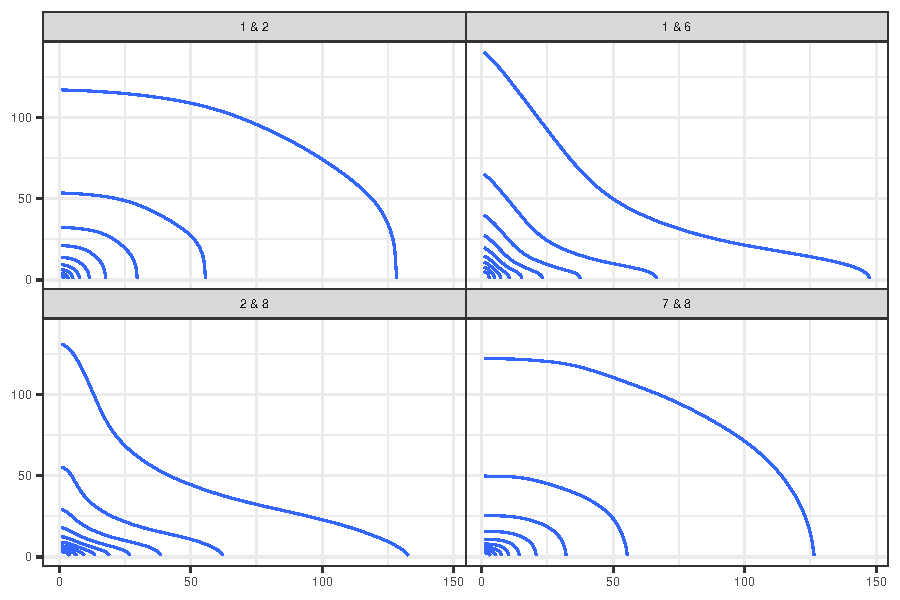
\includegraphics{./images/condsurv_2d}
  \caption{
    Selected bi-variate conditional survival surfaces in extreme regions for the 8 cell data.
    The DP mixture of projected restricted Gammas model was used to generate these surfaces.
  }
\end{figure}










% EOF


\section{Applications to Anomaly Detection}
\subsection{Background}
Anomaly detection describes a field of methods for identifying observations as \emph{anomalous}.  That
  is to say, observations which do not fit the general distribution of the data from which they came.
  Equivalent names for this field are \emph{outlier detection}, and \emph{novelty detection}, though
  some authors in this field will separate the use of those terms by whether or not it is assumed
  that anomalous observations are included in the training dataset.  Crucial to this distinction is
  the existence of a labelled training data set, so that one could effect supervised learning.

For our purpose, we do not assume the existence of labels in the training dataset, and seek an
  algorithm that can produce anomaly scores in the absence of class labels. As such, we will offer
  a brief overview of unsupervised anomaly detection methods, as well as discussion of the methods
  we are preparing here as competing models.

\subsubsection{Statistical Models}
Common to most methods of anomaly detection is the belief that data in regions of relative data sparsity
  are more likely to be anomalous.   To find these regions of sparsity--or more accurately, to find
  which observations are in these regions of sparsity--we generate models to describe the distributional
  density around each observation.  Observations in region of low estimated density are more likely to
  be anomalous.  This subfield includes all manner of non-parametric kernel density estimation such
  as binned histograms, Parzen window methods, along with parametric methods.

\subsubsection{Clustering Methods}
Clustering methods tend to sort data into groups \emph{near} each-other.  These rely on \emph{distance}
  metrics and tend to make no assumptions regarding the underlying distribution of the data.  We can
  further sub-divide this sub-field into density-based, centroid-based, and linkage-based clustering
  methods.

Linkage-based clustering methods group data based on pairwise distance point-to-point, or between
  elements of clusters.  An illustrative example is single linkage, where the distance between two
  clusters is defined as the minimum distance between a point in each set.   Similarly, complete
  linkage defines the metric to be the maximum pairwise between a point in each set. \findcite

Centroid based clustering methods such as $k$-Means instead generate $k$ cluster centroids according
  to some metric, then an observation's \emph{anomaly} score is a function of the distance from that
  observation to the nearest cluster centroid.  More advanced clustering algoritms will look at
  distance to nearest edge, or some combination thereof.  The algorithm used to find the cluster
  centroids is also variable, changing what metric is optimized in finding the location of the
  centroids.  In this subfield, we find the aforementioned $k$-means.

Density based methods will use pairwise distances to establish some measure of local density, then
  establish local modes as clusters.  \emph{DBSCAN} \citep{ester1996} follows this, by forming
  neighborhoods of observations and establishing labels based on the neighborhood.

\subsubsection{Non-Statistical Models}
There are additional non-statistical families of methods beyond clustering, adapted from the realm
  of general classification models to unsupervised learning.  The Isolation Forest,\citep{liu2000}
  adapted from random forests~\citep{breiman2001} uses decision trees to isolate observations.  Those
  observations that are more easily isolable are regarded as more anomalous.  One-class SVM is a
  variant of the support vector machine classification system, where instead of optimizing a
  decision boundary between labelled data, it wraps observed data in a decision boundary.  The
  anomaly score details how close an observation comes to the decision boundary.


\section{Scaling to higher dimensions}
\label{sec:scale}
Under the DP mixture of projected Gammas model detailed in Equation~\ref{eqn:infmixp}, computational
  cost of inference using an MCMC sampler as described scales at $n\log n$ with regard to the number
  of observations under consideration, and linearly with regard to the number of dimensions.  This cost
  is exacerbated in the described model by the need to perform inference steps sequentially.  This is
  alleviated somewhat in the finite mixture model in Equation~\ref{eqn:fmixp}, where cost of inference scales
  linearly with regard to both number of observations, and number of dimensions.  Additionally, inference
  steps can be accomplished in parallel.  For these reasons, for a DP model of a given level of performance,
  an equivalently performant finite mixture model will be \emph{faster} to fit.  But even then, for
  computational cost to increase linearly with the number of dimensions, this will to some extent limit
  our ability to conduct inference at large scale.

To motivate the topic of inference at scale, we consider the topic of storm surge.  Innundation, or
  \emph{flooding} can occur as a result of storm activity--winds as a result of the storm pushing water
  on-shore.  This is exacerbated by current tides, and potentially precipitation as a result of the storm.
  With this in mind, designing levees to protect communities and infrastructure will require an
  understanding of what height storm surge can potentially reach.  Simulated data from
  \emph{SLOSH}~\citep{jelesnianski1992} provide information on inundation scenarios, given parameters
  governing the storm as well as local topological features.  An \emph{observation} from a simulation
  run provides the maximum observed level of storm surge at each site, for potentially millions of sites;
  and there are thousands of available simulation runs.  Even subsetting the data to important
  infrastructure will still yield potentially hundreds of thousands of sites \citep{hutchings2021}.

Scaling our models to this level given our current methods of inference is not feasible, both in
  computational complexity given linear scaling, and in model fidelity.   To control computational
  complexity, one option available to us is an alternative inference algorithm such as variational
  Bayes.~\cite{green2015}.  This works by, in relation to our target model, creating an analogous
  variational model that is \emph{easy} to fit, and inference from this model will come as close as
  possible to our chosen model.  This is generally done by minimizing the K.L. divergence between
  the variational distribution and the target distribution.  This presents a difficulty, as it will
  require evaluation of a density on $\mathcal{S}_{\infty}^{d-1}$.

Model fidelity at high dimensions also presents a difficulty--as we observed in
  Figures~\ref{fig:simes,fig:simppl}, the model performance as measured by energy score for the
  Gamma-based models tends to converge as the number of dimensions grows.  We also observed less
  extant clusters on average on the higher-dimensional data, indicating less ability to identify clusters.
  Given this, one method we believe offers some promise for mantaining model fidelity in high dimensions
  would be a more informative prior for the shape parameter.  In Table~\ref{tab:dev}, we saw the
  log-normal prior for the shape parameters dramatically improve model performance on the real data
  in the higher-dimension case.  If we are using an alternative inference method, then the additional
  computational cost from a more complex prior may be alleviated.

% EOF



\section{Conclusion}
Thus far, we have built upon the definition of the multivariate Pareto described in \cite{ferreira2014}
  to establish a useful parametric representation of its dependence structure, through describing the distribution of its angular component; it being supported on the positive orthant of the unit 
  hypersphere under the $\mathcal{L}_{\infty}$ norm, $\mathcal{S}_{\infty}^{d-1}$.  We then demonstrated an
  inherent difficulty in establishing a distribution supported in this space.  To build that representation,
  we presented a distribution based on a product of independent Gammas, projected onto a supporting manifold
  $\mathcal{S}_{p}^{d-1}$, which will converge to $\mathcal{S}_{\infty}^{d-1}$ as $p\to\infty$.  We then
  established a means of model comparison on $\mathcal{S}_{\infty}^{d-1}$ through the use of a negative
  definite kernel defined in that space.

We used integrated vapor transport data--a measure of water in the atmosphere--as a motivating example for
  our model.  This data subsets California into a series of grid cells, and provides daily IVT values for
  each cell.  We used our model to develop measures of pairwise extremal dependence between grid cells, which
  could be of interest to researchers, actuaries, hydrologists and even farmers.  We additionally developed
  conditional survival functions--$\text{P}\left[Z_l > z_l\mid Z_{\not l} > z_{\not l}\right]$--which provide a more complete understanding of the dependence structure.  The reciprocal of these values provides the more well known \emph{return rates}.

We intend to leverage the information provided to us by our distribution of the angular component to build
  an efficient anomaly detection algorithm.  We have developed a preliminary analysis of two ideas for
  anomaly detection--one based on nearest neighbors, the other based on the posterior predictive loss criterion--and found them to be competitive with existing methods.  We expect development of this topic to take 4 to 6 months.

We finally intend to explore computational developments towards application of our model on large scale
  problems.  We find a motivating example on this topic in simulated storm-surge data, where the length of 
  a data vector can be hundreds of thousands to millions of elements long.  This topic features a pitfall in the curse of dimensionality: with current gamma or log-normal priors, model fidelity drops as the number of dimensions grows.  However, we believe a clever choice of priors for mixture components may improve model fidelity at high dimensions.  We expect development of this topic to completion to take an additional 6-8 months.

% EOF


\newpage

\bibliographystyle{apalike}
\bibliography{./refs}

\end{document}
